% Options for packages loaded elsewhere
\PassOptionsToPackage{unicode}{hyperref}
\PassOptionsToPackage{hyphens}{url}
\PassOptionsToPackage{dvipsnames,svgnames,x11names}{xcolor}
%
\documentclass[
  letterpaper,
  DIV=11,
  numbers=noendperiod]{scrartcl}

\usepackage{amsmath,amssymb}
\usepackage{iftex}
\ifPDFTeX
  \usepackage[T1]{fontenc}
  \usepackage[utf8]{inputenc}
  \usepackage{textcomp} % provide euro and other symbols
\else % if luatex or xetex
  \usepackage{unicode-math}
  \defaultfontfeatures{Scale=MatchLowercase}
  \defaultfontfeatures[\rmfamily]{Ligatures=TeX,Scale=1}
\fi
\usepackage{lmodern}
\ifPDFTeX\else  
    % xetex/luatex font selection
  \setmainfont[]{Times New Roman}
\fi
% Use upquote if available, for straight quotes in verbatim environments
\IfFileExists{upquote.sty}{\usepackage{upquote}}{}
\IfFileExists{microtype.sty}{% use microtype if available
  \usepackage[]{microtype}
  \UseMicrotypeSet[protrusion]{basicmath} % disable protrusion for tt fonts
}{}
\makeatletter
\@ifundefined{KOMAClassName}{% if non-KOMA class
  \IfFileExists{parskip.sty}{%
    \usepackage{parskip}
  }{% else
    \setlength{\parindent}{0pt}
    \setlength{\parskip}{6pt plus 2pt minus 1pt}}
}{% if KOMA class
  \KOMAoptions{parskip=half}}
\makeatother
\usepackage{xcolor}
\setlength{\emergencystretch}{3em} % prevent overfull lines
\setcounter{secnumdepth}{-\maxdimen} % remove section numbering
% Make \paragraph and \subparagraph free-standing
\ifx\paragraph\undefined\else
  \let\oldparagraph\paragraph
  \renewcommand{\paragraph}[1]{\oldparagraph{#1}\mbox{}}
\fi
\ifx\subparagraph\undefined\else
  \let\oldsubparagraph\subparagraph
  \renewcommand{\subparagraph}[1]{\oldsubparagraph{#1}\mbox{}}
\fi


\providecommand{\tightlist}{%
  \setlength{\itemsep}{0pt}\setlength{\parskip}{0pt}}\usepackage{longtable,booktabs,array}
\usepackage{calc} % for calculating minipage widths
% Correct order of tables after \paragraph or \subparagraph
\usepackage{etoolbox}
\makeatletter
\patchcmd\longtable{\par}{\if@noskipsec\mbox{}\fi\par}{}{}
\makeatother
% Allow footnotes in longtable head/foot
\IfFileExists{footnotehyper.sty}{\usepackage{footnotehyper}}{\usepackage{footnote}}
\makesavenoteenv{longtable}
\usepackage{graphicx}
\makeatletter
\def\maxwidth{\ifdim\Gin@nat@width>\linewidth\linewidth\else\Gin@nat@width\fi}
\def\maxheight{\ifdim\Gin@nat@height>\textheight\textheight\else\Gin@nat@height\fi}
\makeatother
% Scale images if necessary, so that they will not overflow the page
% margins by default, and it is still possible to overwrite the defaults
% using explicit options in \includegraphics[width, height, ...]{}
\setkeys{Gin}{width=\maxwidth,height=\maxheight,keepaspectratio}
% Set default figure placement to htbp
\makeatletter
\def\fps@figure{htbp}
\makeatother
\newlength{\cslhangindent}
\setlength{\cslhangindent}{1.5em}
\newlength{\csllabelwidth}
\setlength{\csllabelwidth}{3em}
\newlength{\cslentryspacingunit} % times entry-spacing
\setlength{\cslentryspacingunit}{\parskip}
\newenvironment{CSLReferences}[2] % #1 hanging-ident, #2 entry spacing
 {% don't indent paragraphs
  \setlength{\parindent}{0pt}
  % turn on hanging indent if param 1 is 1
  \ifodd #1
  \let\oldpar\par
  \def\par{\hangindent=\cslhangindent\oldpar}
  \fi
  % set entry spacing
  \setlength{\parskip}{#2\cslentryspacingunit}
 }%
 {}
\usepackage{calc}
\newcommand{\CSLBlock}[1]{#1\hfill\break}
\newcommand{\CSLLeftMargin}[1]{\parbox[t]{\csllabelwidth}{#1}}
\newcommand{\CSLRightInline}[1]{\parbox[t]{\linewidth - \csllabelwidth}{#1}\break}
\newcommand{\CSLIndent}[1]{\hspace{\cslhangindent}#1}

\usepackage{hyperref}

% customize figure references
\renewcommand{\figureautorefname}{Fig.}

% toggle line numbers
\usepackage{lineno}
\linenumbers

% toggle spacing
\usepackage{setspace}
\singlespacing
% \doublespacing

% Hawaiian language characters
% https://tex.stackexchange.com/questions/424535/how-to-type-a-proper-hawai%CA%BBian-%CA%BBokina
\usepackage[utf8]{inputenc}
\usepackage{newunicodechar,graphicx}

\DeclareRobustCommand{\okina}{%
  \raisebox{\dimexpr\fontcharht\font`A-\height}{%
    \scalebox{0.8}{`}%
  }%
}
\newunicodechar{ʻ}{\okina}

% make better hyphen for numeric ranges, \numrange{}{}
\usepackage[detect-none]{siunitx}
\sisetup{range-phrase = \text{--}}
\usepackage{booktabs}
\usepackage{longtable}
\usepackage{array}
\usepackage{multirow}
\usepackage{wrapfig}
\usepackage{float}
\usepackage{colortbl}
\usepackage{pdflscape}
\usepackage{tabu}
\usepackage{threeparttable}
\usepackage{threeparttablex}
\usepackage[normalem]{ulem}
\usepackage{makecell}
\usepackage{xcolor}
\KOMAoption{captions}{tableheading}
\addtokomafont{disposition}{\rmfamily}
\RedeclareSectionCommand[
  font=\normalfont\Large]{section}
\RedeclareSectionCommand[
  font=\normalfont\normalsize\bfseries]{subsection}
\RedeclareSectionCommand[
  font=\normalfont\normalsize\itshape]{subsubsection}
\RedeclareSectionCommand[
  font=\normalfont\normalsize]{paragraph}
\makeatletter
\makeatother
\makeatletter
\makeatother
\makeatletter
\@ifpackageloaded{caption}{}{\usepackage{caption}}
\AtBeginDocument{%
\ifdefined\contentsname
  \renewcommand*\contentsname{Table of contents}
\else
  \newcommand\contentsname{Table of contents}
\fi
\ifdefined\listfigurename
  \renewcommand*\listfigurename{List of Figures}
\else
  \newcommand\listfigurename{List of Figures}
\fi
\ifdefined\listtablename
  \renewcommand*\listtablename{List of Tables}
\else
  \newcommand\listtablename{List of Tables}
\fi
\ifdefined\figurename
  \renewcommand*\figurename{Figure}
\else
  \newcommand\figurename{Figure}
\fi
\ifdefined\tablename
  \renewcommand*\tablename{Table}
\else
  \newcommand\tablename{Table}
\fi
}
\@ifpackageloaded{float}{}{\usepackage{float}}
\floatstyle{ruled}
\@ifundefined{c@chapter}{\newfloat{codelisting}{h}{lop}}{\newfloat{codelisting}{h}{lop}[chapter]}
\floatname{codelisting}{Listing}
\newcommand*\listoflistings{\listof{codelisting}{List of Listings}}
\makeatother
\makeatletter
\@ifpackageloaded{caption}{}{\usepackage{caption}}
\@ifpackageloaded{subcaption}{}{\usepackage{subcaption}}
\makeatother
\makeatletter
\@ifpackageloaded{tcolorbox}{}{\usepackage[skins,breakable]{tcolorbox}}
\makeatother
\makeatletter
\@ifundefined{shadecolor}{\definecolor{shadecolor}{rgb}{.97, .97, .97}}
\makeatother
\makeatletter
\makeatother
\makeatletter
\makeatother
\ifLuaTeX
  \usepackage{selnolig}  % disable illegal ligatures
\fi
\IfFileExists{bookmark.sty}{\usepackage{bookmark}}{\usepackage{hyperref}}
\IfFileExists{xurl.sty}{\usepackage{xurl}}{} % add URL line breaks if available
\urlstyle{same} % disable monospaced font for URLs
\hypersetup{
  pdftitle={Amphistomy increases leaf photosynthesis more in coastal than montane plants of Hawaiian ʻilima (Sida fallax)},
  colorlinks=true,
  linkcolor={blue},
  filecolor={Maroon},
  citecolor={Blue},
  urlcolor={Blue},
  pdfcreator={LaTeX via pandoc}}

\title{Amphistomy increases leaf photosynthesis more in coastal than
montane plants of Hawaiian ʻilima (\emph{Sida fallax})}
\author{}
\date{}

\begin{document}
\maketitle
\ifdefined\Shaded\renewenvironment{Shaded}{\begin{tcolorbox}[borderline west={3pt}{0pt}{shadecolor}, frame hidden, interior hidden, sharp corners, enhanced, breakable, boxrule=0pt]}{\end{tcolorbox}}\fi

\begin{center}
Genevieve Triplett$^1$, Thomas N. Buckley$^2$, Christopher D. Muir$^{1,3,*}$
\end{center}

\(^1\) School of Life Sciences, University of Hawaiʻi Mānoa, Honolulu,
HI, USA 96822

\(^2\) Department of Plant Sciences, University of California, Davis,
CA, USA 95616

\(^3\) Department of Botany, University of Wisconsin, Madison, WI, USA
53706

\(^*\) Corresponding author: Christopher D. Muir, cdmuir@wisc.edu

Manuscript received \_\_\_\_\_\_\_; revision accepted \_\_\_\_\_\_\_.

Running head: Amphistomy advantage in ʻilima

\newpage

\hypertarget{abstract}{%
\section{ABSTRACT ---}\label{abstract}}

\noindent \textbf{Premise of the study} The adaptive significance of
stomata on both upper and lower leaf surfaces, called amphistomy, is
unresolved. A widespread association between amphistomy and open, sunny
habitats suggests the adaptive benefit of amphistomy may be greatest in
these contexts, but this hypothesis has not been tested experimentally.
Understanding amphistomy informs its potential as a target for crop
improvement and paleoenvironment reconstruction.

\textbf{Methods} We developed a method to quantify ``amphistomy
advantage'', \(\mathrm{AA}\), as the log-ratio of photosynthesis in an
amphistomatous leaf to that of the same leaf but with gas exchange
blocked through the upper surface (pseudohypostomy). Humidity modulated
stomatal conductance and thus enabled comparing photosynthesis at the
same total stomatal conductance. We estimated \(\mathrm{AA}\) and leaf
traits in six coastal (open, sunny) and six montane (closed, shaded)
populations of the indigenous Hawaiian species ʻilima (\emph{Sida
fallax}).

\textbf{Key results} Coastal ʻilima leaves benefit 4.04 times more from
amphistomy than montane leaves. Evidence was equivocal with respect to
two hypotheses -- that coastal leaves benefit more because 1) they are
thicker and have lower CO\(_2\) conductance through the internal
airspace, and 2) that they benefit more because they have similar
conductance on each surface, as opposed to most conductance being
through the lower surface.

\textbf{Conclusions} This is the first direct experimental evidence that
amphistomy increases photosynthesis, consistent with the hypothesis that
parallel pathways through upper and lower mesophyll increase CO\(_2\)
supply to chloroplasts. The prevalence of amphistomatous leaves in open,
sunny habitats can partially be explained the increased benefit of
amphistomy in `sun' leaves, but the mechanistic basis remains uncertain.

\textbf{Keywords:} amphistomy, Hawaiʻi, leaf, light, Malvaceae,
photosynthesis, \emph{Sida fallax}, stomata

\hypertarget{introduction}{%
\section{INTRODUCTION ---}\label{introduction}}

Amphistomy, the presence of stomata on both lower and upper surfaces of
broad leaves, should increase carbon gain by reducing the average
diffusion pathlength between stomata and chloroplasts, yet paradoxically
this seemingly simple adaptation is uncommon in nature and we don't know
why. Understanding variation in stomatal traits like amphistomy is
imperative because these tiny pores play an outsized ecological role in
the global carbon and water cycles (Hetherington and Woodward, 2003;
Berry et al., 2010). A widely applicable, accurate representation of how
stomata mediate the relationship between CO\(_2\) gained through
photosynthesis and water lost through transpiration is essential to
predict future climate using Earth Systems Models (Jarvis, 1976; Ball et
al., 1987; Collatz et al., 1991; Leuning, 1995; Sellers et al., 1997).
Optimality models accurately predict the major cause of water loss,
stomatal conductance (\(g_\mathrm{sw}\)), by assuming plants maximize
carbon gain minus a cost of water (Cowan and Farquhar, 1977; Givnish,
1986; Medlyn et al., 2011; Lin et al., 2015; Wang et al., 2017; Franks
et al., 2018; Deans et al., 2020; Franklin et al., 2020; Wang et al.,
2020; Harrison et al., 2021). Despite the success of optimality modeling
in predicting \(g_\mathrm{sw}\), the same modeling approach has so far
failed to explain the rarity of amphistomatous leaves (Muir, 2019).
\textbf{This gap between theory and observations strongly implies that
we remain ignorant about some key benefits and costs associated with
stomata.}

Where are amphistomatous leaves found and why aren't they more common?
Among terrestrial flowering plants, amphistomatous leaves are rarely
found on woody plants and shade-tolerant herbs, but they are common in
annual and perennial herbs from sunny habitats (Salisbury, 1928;
Parkhurst, 1978; Mott et al., 1982; Peat and Fitter, 1994; Gibson, 1996;
Jordan et al., 2014; Muir, 2015, 2018; Bucher et al., 2017). Even in
resupinate leaves where the abaxial surface faces up toward the sky,
stomata develop on the lower adaxial surface (Lyshede, 2002). Exceptions
to this general pattern include some arid woody plants which typically
have vertically oriented, isobilateral leaves (Wood, 1934; Jordan et
al., 2014; Boer et al., 2016; Drake et al., 2019) and
floating/amphibious leaves of aquatic plants (Kaul, 1976; Doll et al.,
2021). The dearth of amphistomatous leaves should be quite surprising
and has been described as one of the most important unsolved problems in
the study of leaf structure-function relations despite some recent
progress (Grubb, 1977, 2020).

Amphistomatous leaves should be common because, all else being equal, a
leaf with a given number of stomata per area could increase its
photosynthetic rate simply by apportioning approximately half its
stomata to each surface (Parkhurst, 1978; Gutschick, 1984a, b). The key
difference between a hypo- and amphistomatous leaf, holding all other
factors constant, is that an amphistomatous leaf has two parallel
diffusion paths through the internal airspace to any given chloroplast.
Those airspaces pose a resistance for CO\(_2\) diffusion, so CO\(_2\)
concentration drops as it approaches chloroplasts. Shorter pathways mean
a smaller drop in CO\(_2\) concentration. Thus, chloroplasts in
amphistomatous leaves experience higher CO\(_2\) concentrations than in
hypostomatous leaves, thereby increasing photosynthesis. The airspace
resistance (or its inverse, the airspace conductance,
\(g_\mathrm{ias}\)) is rarely measured directly and there is
disagreement between empirical (Parkhurst and Mott, 1990; Morison et
al., 2005; Evans et al., 2009; Tomás et al., 2013; Earles et al., 2018;
Šantrůček et al., 2019; Nobel, 2020; Harwood et al., 2021; Márquez et
al., 2023) and theoretical models (Tholen and Zhu, 2011; Ho et al.,
2016; Théroux-Rancourt et al., 2021). The \(g_\mathrm{ias}\) in thin,
porous leaves may be so large as to be inconsequential given much lower
conductances for other components of the diffusion pathway, whereas the
\(g_\mathrm{ias}\) of thick leaves with little airspace may greatly
hinder CO\(_2\) diffusion to chloroplasts. Amphistomy should confer the
largest photosynthetic benefit in leaves with intrinsically low
\(g_\mathrm{ias}\). The airspace conductance is one component of the
overall mesophyll conductance, \(g_\mathrm{m}\), which is often strongly
influenced by the chloroplast surface area exposed to airspace and
mesophyll cell wall thickness (Evans et al., 2009; Gago et al., 2020;
Flexas et al., 2021). Hence, thicker leaves may compensate for lower
\(g_\mathrm{ias}\) through increased chloroplast surface area exposed to
airspace (Terashima et al., 2006), but will still benefit from
amphistomy as long as \(g_\mathrm{ias}\) is finite.

Amphistomy should also enhance photosynthesis when leaf boundary layer
resistance is high, because apportioning total flux between two boundary
layers rather than one results in a smaller CO\(_2\) concentration drop
between the atmosphere and stomata. A similar effect has been validated
with a computer model and measurements for transpiration: amphistomatous
leaves lose somewhat more water for the same vapor pressure deficit and
total \(g_\mathrm{sw}\) (Foster and Smith, 1986), but the additional
carbon gain should be enough to offset this cost under most realistic
conditions (Muir, 2019). However, if minimal stomatal conductance is
related to stomatal density (Drake et al., 2013; Márquez et al., 2022)
and the upper boundary layer conductance is higher, then amphistomy
could cause additional, unavoidable water loss.

The most promising adaptive hypothesis is that amphistomy is important
for maximizing photosynthetic rate under high light. Mott et al. (1982)
proposed that ``plants with a high photosynthetic capacity, living in
full-sun environments, and experiencing rapidly fluctuating or
continuously available soil water'' would benefit most, in terms of
increased carbon gain, from having amphistomatous leaves. As described
above, herbs from sunny habitats are often amphistomatous. Most
variation in stomatal density ratio (\(\mathrm{SR}\), the ratio of
stomatal density between the upper and lower surfaces) among species is
assumed to be genetic, but there is also putatively adaptive plasticity
in response to light. Leaves of \emph{Ambrosia cordifolia}, a desert
perennial herb, are hypostomatous under low light (photosynthetic photon
flux density, PPFD = 110 \(\mu \text{mol}~\text{m}^{-2}~\text{s}^{-1}\))
but develop \textasciitilde20\% of their stomata on the upper surface
under high light (1700 \(\mu \text{mol}~\text{m}^{-2}~\text{s}^{-1}\))
(Mott and Michaelson, 1991). Similarly, \emph{Solanum lycopersicum}
leaves are hypostomatous when grown in the shade but develop
\textasciitilde20\% of their stomata on the upper surface grown under
high light-intensity (Gay and Hurd, 1975). Adult leaves of
\emph{Eucalyptus globulus} are amphistomatous, but the proportion of
adaxial stomata increases from \textasciitilde10-20\% under low light to
\textasciitilde30-40\% under high light (James and Bell, 2001). In
summary, both genetic and plastic responses evince a widespread
association between light and \(\mathrm{SR}\).

The association between high light and amphistomy suggests that `sun'
leaves have the most to gain in terms of increased photosynthesis from
having stomata on both surfaces, as Mott et al. (1982) hypothesized.
Parkhurst (1978) proposed quantifying this benefit as `amphistomy
advantage' (\(\mathrm{AA}\)), which we adopt here with some modification
(see Materials and Methods). This hypothesis has never been tested
directly by comparing the photosynthetic rate of an amphistomatous leaf
to that of an otherwise identical hypostomatous leaf with the same total
stomatal conductance under the same conditions. We propose a
straightforward method to do this by experimentally creating a
pseudohypostomatous leaf with gas exchange blocked through the upper
surface (see Materials and Methods). We use humidity to modulate
stomatal conductance so that amphi- and pseudohypostomatous leaves can
be compared at the same total stomatal conductance. One reason that sun
leaves might have greater \(\mathrm{AA}\) is that they are usually
thicker or denser (Poorter et al., 2019), which will often result in
lower \(g_\mathrm{ias}\) either by increasing the diffusion path length
(Parkhurst, 1978) or making the airspace less porous. A nonmutually
exclusive hypothesis is that if sun leaves have a stomatal density ratio
closer to 0.5 (same density on each leaf surface), this will confer a
greater advantage than an amphistomatous leaf with most stomata on one
surface. In other words, amphistomy doesn't make much difference if one
leaf surface has few open stomata on it. We therefore predict that sun
leaves will have greater \(\mathrm{AA}\) possibly because they have
thicker leaves and/or \(\mathrm{SR}\) closer to 0.5. We actually report
\(g_{\mathrm{smax,ratio}}\), which is similar to \(\mathrm{SR}\) except
that it accounts for differences in both stomatal density and size
between surfaces.

The native flora of the Hawaiian archipelago is a excellent system to
test the relationship between light habitat and \(\mathrm{AA}\). Many
lineages have adapted to different light habitats after colonization and
leaf anatomical traits such as \(\mathrm{SR}\) and thickness vary within
and among closely related species. It is hypothesized that the common
ancestor in many Hawaiian clades was a weedy species with high dispersal
ability adapted to open habitats (Carlquist, 1966). Colonization was
followed by adaptive radiation into higher elevation, montane, closed,
forested habitats. Consequently, adaptation to sun and shade is a common
axis of phenotypic variation among Hawaiian plants such as lobeliads
(Givnish et al., 2004; Montgomery and Givnish, 2008; Givnish et al.,
2009; Givnish and Montgomery, 2014; Scoffoni et al., 2015),
\emph{Bidens} (Carlquist, 1966; Knope et al., 2020), \emph{Scaevola}
(Robichaux and Pearcy, 1984; McKown et al., 2016), \emph{Euphorbia}
(Sporck, 2011), and \emph{Plantago} (Dunbar-Co et al., 2009).

Here we focus on variation within an indigenous plant species \emph{Sida
fallax} Walp. (Malvaceae), known in the Hawaiian language as ʻilima.
ʻIlima is found from sea level to elevations \(>1000\) mas on multiple
Hawaiian islands. Coastal populations are morphologically different from
montane populations (\autoref{fig:study-system}). Coastal regions of
Hawaiʻi are characterized by high sun exposure, warmer temperatures,
high winds, salinity, and variation in water availability. Coastal
populations of ʻilima tend to be short and prostrate which likely helps
them to withstand the windy environment (\autoref{fig:study-system}a).
The leaves of these populations are covered on both surfaces in dense,
soft hairs that give the leaves a silvery green appearance
(\autoref{fig:study-system}b), which helps mitigate water loss by
reflecting solar radiation, thereby lowering leaf temperature
(Ehleringer and Björkman, 1978). Montane regions, on the other hand,
provide very different challenges. Many other tall species grow on the
slopes of these wet mountainous regions, which makes light competition a
factor that plants may need to adapt to. Possibly due to this, montane
populations are erect and shrub- or tree-like, capable of growing meters
tall with strong, woody stems. These individuals have smooth, green
foliage with serrated edges. Montane populations exhibit traits that may
help them to compete for light availability. This montane morphology is
not found in \emph{S. fallax} populations on other Pacific Islands
(Pejhanmehr et al., 2023).

Because of their contrasting habitat and morphology, we treat leaves
from coastal and montane plants as representatives of sun and shade
leaves, respectively, for testing hypotheses about amphistomy advantage.
Specifically, the objectives of our study are to test whether 1) sun
leaves of coastal ʻilima plants will have greater \(\mathrm{AA}\) than
shade leaves of montane plants; and if so, is this because 2a) coastal
plants have thicker leaves than montane plants and/or 2b) coastal plants
have a \(g_{\mathrm{smax,ratio}}\) closer to 0.5?

\hypertarget{methods}{%
\section{MATERIALS AND METHODS ---}\label{methods}}

\hypertarget{plant-sampling}{%
\subsection{Plant sampling and climate ---}\label{plant-sampling}}

We identified 7 suitable natural populations of ʻilima on Oʻahu and 5 on
Hawaiʻi Island by consulting Yorkston and Daehler (2006) and citizen
scientist records on iNaturalist (Anon, 2022)
(\autoref{fig:study-system}c; \autoref{tbl-locations}). We avoided sites
that appeared to be cultivated. We visited sites between August and
November 2022. For logistical reasons, the sites on Hawaiʻi were sampled
during one three-day trip. We haphazardly sampled eight plants
distributed evenly between the highest and lowest elevation plants along
a transect at each site. For safety and conservation reasons, transects
were along a trail or road. We did not sample small individuals if there
was risk removing leaves would cause mortality. From each plant, we
collected two fully expanded leaves for trait measurements. We sampled
stomatal traits on all leaves; leaf thickness on one leaf from three
randomly selected plants per site; and, due to limited time, a single
leaf from a single plant at the middle of each transect for gas exchange
measurements. We downloaded climatic data on mean annual temperature,
solar radiation, and vegetation height from the Climate and Solar
Radiation of Hawaiʻi databases (Giambelluca et al., 2014) using the
latitude and longitude at the middle of each transect. We also
downloaded mean annual precipitation from 1978-2007 from the Rainfall
Atlas of Hawaiʻi (Giambelluca et al., 2013). The spatial resolution is
approximately \(234 \times 250\)m. The temperature data are calibrated
from networks of meteorological stations operating in the late 20th
century and 21st century; the solar radiation data are calibrated from
satellite measurements collected between 2002 and 2009 (Giambelluca et
al., 2014). We tested whether climatic variables differed among our
coastal and montane populations using Welch's two-sample \(t\)-test.

\hypertarget{leaf-traits}{%
\subsection{Leaf traits ---}\label{leaf-traits}}

\hypertarget{stomata}{%
\subsubsection{Stomata ---}\label{stomata}}

We estimated the stomatal density and size on ab- and adaxial leaf
surfaces from all leaves. For pubescent leaves (usually coastal), we
dried and pressed leaves for \(\approx 1\) week (Hill et al., 2014),
carefully scraped trichomes off with a razor blade, and rehydrated the
leaf. Rehydration restores leaf area to its fresh value (Blonder et al.,
2012). For glabrous leaves, we used fresh leaves. We applied clear nail
polish to both leaf surfaces of fresh or rehydrated leaves in the middle
of the lamina away from major veins. After nail polish dried, we mounted
impressions on a microscope slide using transparent tape (Mott and
Michaelson, 1991). We digitized a portion of each leaf surface
impression using a brightfield microscope (Leica DM2000, Wetzlar,
Germany). We counted all stomata and divided by the visible leaf area
(0.890 mm\(^2\)) to estimate density and measured guard cell length from
five randomly chosen stomata per field using ImageJ (Schneider et al.,
2012).

\hypertarget{leaf-thickness}{%
\subsubsection{Leaf thickness ---}\label{leaf-thickness}}

We cut thin sections using two razor blades taped together. We sectioned
the leaf in a petri dish of water, wet-mounted sections onto a slide,
and took digital micrographs using a brightfield microscope, as
described above. Leaf thickness is measured as the length from upper
cuticle to lower cuticle.

\hypertarget{gas-exchange-measurements}{%
\subsubsection{Gas exchange measurements
---}\label{gas-exchange-measurements}}

At each site, we selected one representative leaf from one plant near
the middle of the transect for gas exchange measurements using a
portable infrared gas analyzer (LI-6800PF, LI-COR Biosciences, Lincoln,
Nebraska, USA). We estimated the photosynthetic rate (\(A\)) and
stomatal conductance to water vapor (\(g_\text{sw}\)) at saturating
light
(\(\text{photosynthetic photon flux density (PPFD)} = 2000~\mu \text{mol}~\text{m}^{-2}~\text{s}^{-1}\)),
ambient CO\(_2\) (415 ppm), and
\(T_\mathrm{leaf} = 25.0 \textendash 29.3° \text{C}\). The midday
irradiance in coastal ʻilima typically meets or even exceeds a PPFD of
\(2000~\mu \text{mol}~\text{m}^{-2}~\text{s}^{-1}\) and previous
experiments with sun leaves revealed that
\(2000~\mu \text{mol}~\text{m}^{-2}~\text{s}^{-1}\) is always at or near
saturating irradiance. Even though lower irradiance may be saturating
for montane leaves, we used this higher value for all leaves to
standardize conditions.

We also estimated `amphistomy advantage' (\(\mathrm{AA}\)) \emph{sensu}
Parkhurst (1978), but with modification. For each leaf, we measured the
photosynthetic rate of an untreated amphistomatous leaf
(\(A_{\mathrm{amphi}}\)) over a range of \(g_\text{sw}\) values. We
refer to this as an \(A \textendash g_\text{sw}\) curve, which is
described in more detail below. We compared the
\(A \textendash g_\text{sw}\) curve of the untreated leaf to the
photosynthetic rate of pseudohypostomatous leaf (\(A_\mathrm{hypo}\)),
which is the same leaf but with gas exchange through the upper surface
blocked by a neutral density plastic (propafilm). Hypostomy refers to
leaves with stomata only present on the lower, typically abaxial,
surface. We refer to the untreated and partially blocked leaves as
``amphi'' and ``pseudohypo'', respectively. \(\mathrm{AA}\) is
calculated as the log-response ratio of \(A\) compared at the same total
\(g_\text{sw}\):

\[\mathrm{AA} = \mathrm{log}(A_{\mathrm{amphi}} / A_{\mathrm{hypo}})\]

The log-response ratio is commonly used social and biological sciences
(e.g. Hedges et al. (1999)). It is straightforward to interpret because
values above 0 indicate a photosynthetic advantage of amphistomy,
whereas values less than 0 indicate a disadvantage. The log-response
ratio is preferable to the absolute difference because it indicates a
proportional change in \(A\), which facilitates comparisons across
leaves and environments with different baseline photosynthetic rates.
The irradiance of the light source in the pseudohypo leaf was higher
because the propafilm reduces transmission. To compensate for reduced
transmission, we increased incident \(\mathrm{PPFD}\) for pseudohypo
leaves by a factor 1/0.91, the inverse of the measured transmissivity of
the propafilm. We also set the stomatal conductance ratio, for purposes
of calculating boundary layer conductance, to 0 for pseudohypo leaves
following manufacturer directions.

Appendix S1 (see the Supplementary Data with this article),
\autoref{fig:ags-curve} illustrates our method for collecting
\(A \textendash g_\text{sw}\) curves. We collected two curves per leaf,
an amphi (untreated) curve and a pseudohypo (treated) curve. To control
for order effects, we alternated between starting with amphi or
pseudohypo leaf measurements, though we did not detect an effect of
treatment order on \(\mathrm{AA}\) (results not shown). In the field, we
acclimated the focal leaf to saturating light and high relative humidity
(\(\mathrm{RH} = 70\%\)), as described above, until \(A\) and
\(g_\text{sw}\) reach their maximum. We used these data as our estimates
of maximum \(A\) and \(g_\text{sw}\). After that, we decreased
\(\mathrm{RH}\) to \(\approx 10\%\) to induce rapid stomatal closure
without biochemical downregulation. Hence, \(A_\text{amphi}\) and
\(A_\text{hypo}\) were both measured at low chamber humidity after the
leaf had acclimated to high humidity. All other environmental conditions
in the leaf chamber remained the same. We logged data until
\(g_\text{sw}\) reached its nadir. We then repeated the process of
acclimating the leaf to 70\% \(\mathrm{RH}\) and inducing stomatal
closure with low \(\mathrm{RH}\) with the other treatment (amphi or
pseudohypo).

\hypertarget{data-analyis}{%
\subsection{Data analysis ---}\label{data-analyis}}

\hypertarget{objective-1-do-coastal-leaves-have-greater-amphistomy-advantage-than-montane-leaves}{%
\subsubsection{Objective 1: Do coastal leaves have greater amphistomy
advantage than montane leaves?
---}\label{objective-1-do-coastal-leaves-have-greater-amphistomy-advantage-than-montane-leaves}}

It is not feasible to record \(A_\mathrm{amphi}\) and
\(A_\mathrm{hypo}\) at the exact same \(g_\text{sw}\). To overcome this,
we fit \(A \textendash g_\text{sw}\) curves using a linear regression of
\(\text{log}(g_\mathrm{sw})\) on \(A\) to interpolate modeled \(A\) for
amphi and pseudohypo leaves at the same \(g_\text{sw}\). Let
\(\hat{A}_\text{amphi}\) and \(\hat{A}_\text{hypo}\) be the estimated
\(A\) of the amphi and pseudohypo leaves, respectively. We estimated
these quantities at the same \(g_\mathrm{sw}\) using fitted parameters
(\(\hat{\beta}\)'s):

\[\hat{A}_\text{amphi} = \hat{\beta}_{0,\text{amphi}} + \hat{\beta}_{1,\text{amphi}} \times \text{log}(g_\mathrm{sw})\]
\[\hat{A}_\text{hypo} = \hat{\beta}_{0,\text{hypo}} + \hat{\beta}_{1,\text{hypo}} \times \text{log}(g_\mathrm{sw})\]

In 10 of 12 leaves, the minimum \(g_\text{sw}\) of the amphi curve was
smaller than the maximum \(g_\text{sw}\) of the pseudohypo curve
(i.e.~the curves overlapped for a range of \(g_\text{sw}\) values). In
those cases, we estimated \(\hat{A}_\text{amphi}\) and
\(\hat{A}_\text{hypo}\) at the \(g_\mathrm{sw}\) value in the middle of
the range of overlap between the curves. In 2 of 12 leaves, the
\(A \textendash g_\text{sw}\) curves did not quite overlap because the
minimum \(g_\text{sw}\) of the amphi curve was slightly greater than the
maximum \(g_\text{sw}\) of the pseudohypo curve. In those cases, we
estimated \(\mathrm{AA}\) by extrapolating slightly,
\(1.98\times 10^{-3}~\text{and}~3.29\times 10^{-3}~\text{mol}~\text{m}^{-2}~\text{s}^{-1}\),
beyond the measured curves to the \(g_\mathrm{sw}\) value in between the
curves. The vertical lines in Appendix S1, \autoref{fig:licor} show the
\(g_\text{sw}\) for each leaf. We estimated \(\mathrm{AA}\) from
\(\hat{A}_\text{amphi}\) and \(\hat{A}_\text{hypo}\) for each leaf using
the log-response ratio shown above.

To estimate \(\hat{\beta}\)'s from the \(A \textendash g_\text{sw}\)
curve for each leaf, we fit Bayesian regressions using the \emph{R}
package \textbf{brms} version 2.20.4 (Bürkner, 2017) with MCMC sampling
in \emph{Stan} (Stan Development Team, 2023). We used CmdStan version
2.33.1 and \textbf{cmdstanr} version 0.6.1 (Gabry et al., 2023) to
interface with \emph{R} version 4.3.1 (R Core Team, 2023). We sampled
the posterior distribution from 4 chains with 1000 iterations each after
1000 warmup iterations per chain. We estimated parameters and confidence
intervals as the median and 95\% quantile intervals of the posterior,
respectively. The key prediction is that
\(\mathrm{AA}_\text{coastal} > \mathrm{AA}_\text{montane}\), meaning the
95\% confidence intervals of
\(\mathrm{AA}_\text{coastal} - \mathrm{AA}_\text{montane}\) should be
positive and not encompass 0.

\hypertarget{objective-2a-are-coastal-leaves-thicker-than-montane-leaves}{%
\subsubsection{Objective 2a: Are coastal leaves thicker than montane
leaves?
---}\label{objective-2a-are-coastal-leaves-thicker-than-montane-leaves}}

We tested whether leaf thickness (log-transformed) varied between
coastal and montane populations and among individuals within populations
using a Bayesian mixed-effects model with habitat as a fixed effect and
individual plant and site as random effects. We used the \emph{R}
package \textbf{brms} version 2.20.4 (Bürkner, 2017) to fit the model in
\emph{Stan} (Stan Development Team, 2023) with CmdStan version 2.33.1
and \textbf{cmdstanr} version 0.6.1 (Gabry et al., 2023). We sampled the
posterior distribution from 4 chains with 1000 iterations each after
1000 warmup iterations per chain. We estimated the relationship between
population average leaf thickness and \(\mathrm{AA}\) measured from a
single individual per population. We used this approach because most of
the variation in leaf thickness was among sites and the plant selected
for gas exchange measurements was not always among the plants randomly
selected for leaf thickness, precluding individual level correlation. We
propagated uncertainty about in \(\mathrm{AA}\) and leaf thickness
estimates by integrating over the entire posterior distribution sample
for each variable. The key prediction is that the effect of leaf
thickness on \(\mathrm{AA}\) is positive, meaning the 95\% confidence
interval of the slope should be positive and not encompass 0.

\hypertarget{objective-2b-is-g_mathrmsmaxratio-closer-to-0.5-in-coastal-leaves-than-montane-leaves}{%
\subsubsection{\texorpdfstring{Objective 2b: Is
\(g_{\mathrm{smax,ratio}}\) closer to 0.5 in coastal leaves than montane
leaves?
---}{Objective 2b: Is g\_\{\textbackslash mathrm\{smax,ratio\}\} closer to 0.5 in coastal leaves than montane leaves? ---}}\label{objective-2b-is-g_mathrmsmaxratio-closer-to-0.5-in-coastal-leaves-than-montane-leaves}}

We tested whether \(g_\mathrm{smax,ratio}\) varied between coastal and
montane populations and among individuals within populations using a
Bayesian mutliresponse, mixed-effects model. The modeled response
variables are stomatal count and guard cell length on each surface.
Counts were modeled as negative binomially distributed variable from a
latent stomatal density and a parameter \(\phi\) to estimate
overdispersion in counts relative to a Poisson model. For all traits,
the explanatory variables were habitat as a fixed effect and leaf within
individual plant, individual plant, and site as random effects. We used
the \emph{R} package \textbf{brms} version 2.20.4 (Bürkner, 2017) to fit
the model in \emph{Stan} (Stan Development Team, 2023) with CmdStan
version 2.33.1 and \textbf{cmdstanr} version 0.6.1 (Gabry et al., 2023).
We interpolated missing adaxial guard cell lengths from 6 out of 185
samples with zero adaxial stomata using the ``mi'' function in
\textbf{brms} package. We sampled the posterior distribution from 4
chains with 1000 iterations each after 1000 warmup iterations per chain.
From each posterior sample, we calculated \(g_{\mathrm{smax,ratio}}\)
as:

\[g_\mathrm{smax,ratio} = \frac{g_\mathrm{smax,upper}}{g_\mathrm{smax,lower} + g_\mathrm{smax,upper}},\]

where \(g_\mathrm{smax,lower}\) and \(g_\mathrm{smax,upper}\) are
maximum stomatal conductance to water vapor at
\(T_\mathrm{leaf} = 25 ^ \circ\) C on the lower and upper surface,
respectively. The maximum stomatal conductance was calculated from
stomatal density and length, assuming that stomata are fully open,
following Sack and Buckley (2016):

\[g_\mathrm{smax} = bmds^{0.5}.\] In this equation, \(b\) is a
biophysical constant, \(m\) is a morphological constant, \(d\) is the
stomatal density, and \(s\) is the stomatal complex area. We assume that
\(b\), which is determined by the molecular species, temperature, and
air pressure, is the same for both surfaces; we assume that \(m\), which
is determined by guard cell allometry is also the same for both
surfaces. Hence, the \(b\) and \(m\) constants cancel out of
\(g_\mathrm{smax,ratio}\) and only density and length (\(l\)), which is
proportional to the square root of area, affect the ratio:
\(g_\mathrm{smax} \propto dl\).

We estimated the relationship between leaf \(g_\mathrm{smax,ratio}\) and
\(\mathrm{AA}\) measured from a single leaf per population. We
propagated uncertainty about \(\mathrm{AA}\) and
\(g_\mathrm{smax,ratio}\) by integrating over the entire posterior
distribution sample for each variable. The key prediction is that the
effect of \(g_\mathrm{smax,ratio}\) on \(\mathrm{AA}\) is positive until
\(g_\mathrm{smax,ratio} < 0.5\), meaning the 95\% confidence interval of
the slope should be positive and not encompass 0 in the domain
\(g_\mathrm{smax,ratio} < 0.5\).

\hypertarget{results}{%
\section{RESULTS ---}\label{results}}

Coastal ʻilima are surrounded by shorter vegetation than their montane
counterparts (\autoref{fig:study-system}d; Welch Two Sample
\emph{t}-test, \(t_{6.67} = 5.13\), \(P = 0.002\)). The montane site
with the lowest vegetation height is a remnant dry forest (Koaiʻa tree
sanctuary) in a matrix of cattle pasture, hence the satellite derived
vegetation height may be lower than what existed prior to human
disturbance. Coastal sites receive greater average solar radiation at
the top of the canopy (\autoref{fig:study-system}d; Welch Two Sample
\emph{t}-test, \(t_{10.86} = -2.22\), \(P = 0.049\)); coastal sites are
significantly warmer (\autoref{fig:study-system}d; Welch Two Sample
\emph{t}-test, \(t_{6.01} = -2.96\), \(P = 0.025\)); and coastal sites
receive less precipitation (\autoref{fig:study-system}d; Welch Two
Sample \emph{t}-test, \(t_{7.45} = 2.73\), \(P = 0.028\)).

\hypertarget{amphistomy-advantage-is-greater-in-coastal-leaves}{%
\subsection{Amphistomy advantage is greater in coastal leaves
---}\label{amphistomy-advantage-is-greater-in-coastal-leaves}}

Amphistomy increases photosynthesis in leaves of coastal ʻilima plants
more than that of montane plants. \(\mathrm{AA}\) was significantly
greater than 0 (95\% confidence intervals did not overlap 0) in 5 of 6
coastal leaves, but only 1 of 6 montane leaves
(\autoref{fig:habitat-aa}; see Appendix S1, \autoref{fig:licor} for
individual curves). Overall, the average \(\mathrm{AA}\) among coastal
and montane leaves is \(0.12~[\numrange{0.077}{0.15}]\) and
\(0.027~[\numrange{-0.0034}{0.057}]\), respectively; the difference in
average \(\mathrm{AA}\) between habitat types is
\(\mathrm{AA}_\text{coastal} - \mathrm{AA}_\text{montane} = 0.09~[\numrange{0.039}{0.14}]\).
Posterior predictions closely match observed values of \(A\) (Appendix
S1, \autoref{fig:pp-licor}), indicating an adequate model fit from which
we can interpolate between measurements reliably. It also suggests that
slight extrapolation beyond the data should be reliable, but this is
less certain. When we remove two leaves where we extrapolated slightly
beyond fitted \(A \textendash g_\mathrm{sw}\) curves, we estimate that
\(\mathrm{AA}_\text{coastal}\) is still positive,
\(0.081~[\numrange{0.023}{0.13}]\), but the difference between coastal
and montane leaves is smaller, \(0.053~[\numrange{-0.012}{0.12}]\), and
confidence intervals slightly overlap 0. Maximum photosynthetic rate was
slightly, but not significantly higher in coastal leaves (Welch Two
Sample \emph{t}-test, \(t_{9.65} = 1.6\), \(P = 0.14\)); total stomatal
conductance was similar (Welch Two Sample \emph{t}-test,
\(t_{9.71} = -0.09\), \(P = 0.93\)) in coastal and montane leaves
(Appendix S1, \autoref{fig:habitat-Ags}). Water-use efficiency
(\(A / g_\mathrm{sw}\)) was significantly higher in coastal leaves
(Welch Two Sample \emph{t}-test, \(t_{9.99} = 2.54\), \(P = 0.03\)).

\hypertarget{leaf-thickness-is-associated-with-amphistomy-advantage-between-but-not-within-habitats}{%
\subsection{Leaf thickness is associated with amphistomy advantage
between but not within habitats
---}\label{leaf-thickness-is-associated-with-amphistomy-advantage-between-but-not-within-habitats}}

Coastal ʻilima leaves are \(91~[\numrange{26}{164}]\) \(\mu\text{m}\)
thicker than their montane counterparts. Although coastal leaves are
thicker and have greater \(\mathrm{AA}\), there is little relationship
between leaf thickness and \(\mathrm{AA}\) within habitats
(\autoref{fig:traits-aa}A;
\(\text{slope}~= -0.11~[\numrange{-0.28}{0.035}]\)).

\hypertarget{g_mathrmsmaxratio-is-not-associated-with-amphistomy-advantage}{%
\subsection{\texorpdfstring{\(g_\mathrm{smax,ratio}\) is not associated
with amphistomy advantage
---}{g\_\textbackslash mathrm\{smax,ratio\} is not associated with amphistomy advantage ---}}\label{g_mathrmsmaxratio-is-not-associated-with-amphistomy-advantage}}

Coastal and montane leaves have similar average
\(g_\mathrm{smax,ratio}\), the ratio of adaxial (upper) to total
\(g_\mathrm{smax}\), the anatomical maximum stomatal conductance to
water vapor (Appendix S1, \autoref{fig:habitat-gmaxratio}); coastal
leaves have \(0.059~[\numrange{-0.14}{0.28}]\) higher
\(g_\mathrm{smax,ratio}\) than montane leaves, but the 95\% confidence
intervals overlap 0 difference. The \(g_\mathrm{smax,ratio}\) is
somewhat bimodal among sites. Some sites in both habitats have leaves
with \(g_\mathrm{smax,ratio} < 0.07\) and others with
\(g_\mathrm{smax,ratio} > 0.2\) (Appendix S1,
\autoref{fig:habitat-gmaxratio}). This is particularly noticeable in
montane sites where those on the Big Island of Hawaiʻi all have low
\(g_\mathrm{smax,ratio}\) whereas those on Oʻahu have relatively high
\(g_\mathrm{smax,ratio}\). There is no relationship between
\(g_\mathrm{smax,ratio}\) and \(\mathrm{AA}\) in either habitat
(\autoref{fig:traits-aa}B;
\(\text{slope}~= 0.14~[\numrange{-0.057}{0.34}]\)) in our sample.

\hypertarget{discussion}{%
\section{DISCUSSION ---}\label{discussion}}

Amphistomy is a seemingly simple way that leaves can increase carbon
gain without significant additional water loss, yet it is rare in nature
and we do not know why. The strong association between amphiostomy and
sunny, open habitats suggests that amphistomy may benefit sun leaves
more than shade leaves, but progress has been limited by the lack of
evidence that amphiostomy \emph{per se} improves photosynthesis in a
given leaf. By experimentally blocking gas exchange through the upper
surface in a controlled environment, we directly compared an
amphistomatous leaf to an otherwise identical pseudohypostomatous leaf.
This allows us to quantity the amphistomy advantage (\(\mathrm{AA}\))
holding all else constant. Taking advantage of the steep climatic
gradients in the Hawaiian archipelago, we applied this new method to
show for the first time that sun leaves benefit 4.04 times more from
amphistomy than shade leaves on ʻilima (\emph{Sida fallax}) plants
(\(\mathrm{AA}_\text{coastal} = 0.12\)
vs.~\(\mathrm{AA}_\text{montane} = 0.027\)). Coastal and montane ʻilima
leaves are likely good representatives of classic sun and shade leaf
syndromes because 1) they vary in traits like reflective pubescence
(Ehleringer and Björkman, 1978) and leaf thickness (Terashima et al.,
2001) that typically characterize sun-shade adaptation; and 2) since
ʻilima shrubs are typically \(<1\)m tall, they are shaded by trees in
montane, but not coastal habitats (\autoref{fig:study-system}d). While
this result has not yet been validated in other species, our results
indicate that part of the reason amphistomatous leaves are found most
commonly in high light habitats is that the adaptive benefit is greater
in such environments.

If \(\mathrm{AA}\) is typically greater in sun leaves than shade leaves,
it could partially explain the distribution of amphi- and hypostoamtous
leaves, but the precise mechanism(s) require further study. One
hypothesis is that the internal airspace conductance,
\(g_\mathrm{ias}\), from stomata to mesophyll cell walls is lower in
thicker sun leaves (Parkhurst, 1978). All else being equal, a leaf with
lower \(g_\mathrm{ias}\) will benefit more from amphistomy. Our results
partially support this hypothesis. Coastal ʻilima leaves with high
\(\mathrm{AA}\) (\autoref{fig:habitat-aa}) are thicker than montane
leaves, but the relationship between \(\mathrm{AA}\) and leaf thickness
within habitats is actually slightly negative
(\autoref{fig:traits-aa}a), opposite our prediction. Since coastal and
montane leaves differ in many respects besides thickness, we do not have
enough data to conclude that leaf thickness explains the variation in
\(\mathrm{AA}\) between habitats. Alternatively, other biochemical or
anatomical differences between coastal and montane leaves may explain
why \(\mathrm{AA}\) is greater in coastal leaves. The negative
relationship, albeit nonsignificant in that 95\% confidence intervals
encompassed 0, between leaf thickness and \(\mathrm{AA}\) could be
explained if thicker leaves compensated by having a more porous
mesophyll and/or less tortuous airspaces (Théroux-Rancourt et al.,
2021).

A second natural hypothesis is that amphistomatous leaves with few
adaxial (upper) stomata benefit less than those with similar densities
on both surfaces. We predicted that leaves with
\(g_\mathrm{smax,ratio}\) closer to 0.5 would have higher
\(\mathrm{AA}\) based on biophysical models (Gutschick, 1984a). The
logic is that a small number of stomata on the upper surface are
insufficient to supply the entire upper mesophyll due to limited lateral
diffusion (Morison et al., 2005). Our results do not support this
hypothesis. Montane leaves from Big Island sites had low
\(g_\mathrm{smax,ratio}\) and low \(\mathrm{AA}\) whereas low montane
leaves on Oʻahu had high \(g_\mathrm{smax,ratio}\), but similarly low
\(\mathrm{AA}\) (\autoref{fig:traits-aa}b). Among coastal sites, the
site with the lowest \(g_\mathrm{smax,ratio}\) had the lowest
\(\mathrm{AA}\), but there was little variation in
\(g_\mathrm{smax,ratio}\) among coastal leaves in our sample. We
therefore cannot rule out that a larger sample of coastal leaves with
greater variance in \(g_\mathrm{smax,ratio}\) might support this
hypothesis.

Two major implications from our study are that 1) photosynthesis in
hypostomatous leaves is likely limited by CO\(_2\) concentration
drawdown within leaf airspaces; and 2) amphistomy \emph{per se}
contributes to, but is not wholly responsible for, higher photosynthetic
rates among amphistomatous leaves. The amphistomy advantage we observe
in ʻilima leaves implies decreased CO\(_2\) supply in
pseudohypostomatous leaves because of concentration drawdowns in the
leaf airspace. Limited diffusion through the airspace has long been
hypothesized to depress photosynthesis in hypostomatous leaves
(Parkhurst, 1994), with empirical support from helox studies (Parkhurst
and Mott, 1990). However, these studies relied on interspecific
comparisons of amphi- and hypostomatous leaves that differ
systematically in many traits that affect gas exchange and
photosynthesis (Xiong and Flexas, 2020). Our experimental approach
overcomes this limitation and implies that the drop in CO\(_2\)
concentration from substomatal cavities to the upper surface depresses
photosynthesis.

Among land plants grown in a common garden, amphistomatous leaves have
on average nearly \(2\times\) higher area-based photosynthetic rates
(Xiong and Flexas, 2020), naively implying an
\(\mathrm{AA} \approx \text{log}~2 = 0.69\). This is much higher than
our estimate of 0.12 among coastal ʻilima leaves. The most likely
explanation is that amphistomy is not the only cause of high
photosynthetic rate. Indeed, species adapted to open, high light
habitats with amphistomatous leaves also have higher concentrations of
Rubisco, overall stomatal conductance, and photosynthetic capacity
(Smith et al., 1997; Xiong and Flexas, 2020). For a leaf with high
photosynthetic capacity that is well illuminated and hydrated, the major
limitation becomes CO\(_2\). Under these conditions, amphistomy may
substantially increase photosynthesis, as we observe in coastal ʻilima
leaves. Selection on increased photosynthesis under similar conditions
may explain why crop leaves tend to increase stomatal density ratio
during domestication (Milla et al., 2013).

Three limitations of this study are the small sample size, experimental
design that precludes distinguishing genetic from environmental
differences in leaf traits, and potentially confounding effects of other
environmental differences besides light environment. Understanding the
mechanistic basis of higher \(\mathrm{AA}\) in sun leaves would require
much larger sample sizes. Sun leaves tend to be thicker, more densely
packed with mesophyll cells, and have greater photosynthetic capacity
and higher stomatal conductance, among other traits (Lambers et al.,
2008). Each of these factors and others potentially modulate
\(\mathrm{AA}\). Quantifying the contribution of all these factors
requires larger samples and additional measurements that are beyond the
scope of this study, but exciting avenues for future research on leaf
structure-function relations. Although many morphological traits that
distinguish coastal and montane ʻilima populations persist in a common
environment (Yorkston and Daehler, 2006), we cannot distinguish between
genetic effects and plastic responses to habitat as causes of difference
in \(\mathrm{AA}\) because we measured naturally occurring plants
\emph{in situ}. While disentangling genetic and plastic contributions is
not necessarily important for understanding the distribution of
amphistomatous leaves, it would be insightful to know about genetic and
environmental contributions to trait variation. A reciprocal transplant
would be able to determine the genetic and environmental contributions,
as well their interaction, to trait variance in nature. However,
reciprocal transplants cannot control for other differences between
coastal and montane habitats besides vegetation height, such as
temperature and precipitaiton. Experimental studies in controlled
environments will be necessary to isolate the effects of light quantity
and quality on \(\mathrm{AA}\).

\hypertarget{conclusions}{%
\section{CONCLUSIONS ---}\label{conclusions}}

This study reports the first direct experimental evidence that having
stomata open on both leaf surfaces, amphistomy, increases photosynthesis
for a given total stomatal conductance, particularly in leaves from the
type of open, sunny habitats where this trait is most common. By
developing a straightforward experimental method to block gas exchange
through the upper surface, we directly compared the photosynthetic rate
of a leaf with gas exchange through both surfaces or just one, holding
all other factors constant. In doing so, we found that coastal leaves of
the indigenous Hawaiian ʻilima (\emph{Sida fallax}) enjoyed a greater
photosynthetic benefit from amphistomy than nearby montane leaves living
in more closed forest. This is not because amphistomatous leaves
necessarily have greater leaf surface available for stomata, although
that likely influences realized photosynthetic rates in natural
populations. Rather, our experiments show that coastal amphistomatous
leaves with the same total leaf stomatal conductance photosynthesize
more than identical hypostomatous leaves. We cannot yet ascribe the
difference in amphistomy advantage between coastal and montane leaves to
particular physiological or anatomical variation, but this is a
promising area for future research.

\hypertarget{acknowledgments}{%
\section{Acknowledgments ---}\label{acknowledgments}}

The authors thank Kasey Barton and three anonymous reviewers for
feedback on an earlier version of this manuscript, the University of
Hawaiʻi honors council for guidance to GT, Tawn Speetjens for access to
one montane site, TM Perez for advice on leaf sectioning, startup funds
from the University of Hawaiʻi, NSF Award 1929167 to CDM, and NSF Award
2307341 to TNB. This is publication \#213 from the School of Life
Sciences, University of Hawaiʻi at Mānoa.

\hypertarget{author-ontributions}{%
\section{Author Contributions ---}\label{author-ontributions}}

GT and CDM contributed equally to all stages of this project; TNB
contributed to development of the method and helped edit the manuscript.

\hypertarget{data-availability-statement}{%
\section{Data Availability Statement
---}\label{data-availability-statement}}

Custom scripts are available on a GitHub repository
(https://github.com/cdmuir/stomata-ilima) and archived on Zenodo
(https://doi.org/10.5281/zenodo.10369114). Raw data are deposited on
Dryad (https://doi.org/10.5061/dryad.rxwdbrvfw ).

\hypertarget{supporting-information}{%
\section{Supporting Information ---}\label{supporting-information}}

Additional supporting information may be found online in the Supporting
Information section at the end of the article.

\begin{itemize}
\tightlist
\item
  Appendix S1: Supplemental figures and table
\end{itemize}

\newpage

\hypertarget{literature-cited}{%
\section{Literature Cited ---}\label{literature-cited}}

\hypertarget{refs}{}
\begin{CSLReferences}{1}{0}
\leavevmode\vadjust pre{\hypertarget{ref-noauthor_inaturalist_2022}{}}%
Anon. 2022. \href{https://www.inaturalist.org}{{iNaturalist}}.

\leavevmode\vadjust pre{\hypertarget{ref-biggins_model_1987}{}}%
Ball, J. T., I. E. Woodrow, and J. A. Berry. 1987.
\href{https://doi.org/10.1007/978-94-017-0519-6_48}{A {Model}
{Predicting} {Stomatal} {Conductance} and its {Contribution} to the
{Control} of {Photosynthesis} under {Different} {Environmental}
{Conditions}}. \emph{In} J. Biggins {[}ed.{]}, Progress in
{Photosynthesis} {Research}, 221--224. Springer Netherlands, Dordrecht.

\leavevmode\vadjust pre{\hypertarget{ref-berry_stomata:_2010}{}}%
Berry, J. A., D. J. Beerling, and P. J. Franks. 2010.
\href{https://doi.org/10.1016/j.pbi.2010.04.013}{Stomata: Key players in
the earth system, past and present}. \emph{Current Opinion in Plant
Biology} 13: 232--239.

\leavevmode\vadjust pre{\hypertarget{ref-blonder_leaf-area_2012}{}}%
Blonder, B., V. Buzzard, I. Simova, L. Sloat, B. Boyle, R. Lipson, B.
Aguilar-Beaucage, et al. 2012.
\href{https://doi.org/10.3732/ajb.1200062}{The leaf-area shrinkage
effect can bias paleoclimate and ecology research}. \emph{American
Journal of Botany} 99: 1756--1763.

\leavevmode\vadjust pre{\hypertarget{ref-de_boer_apparent_2016}{}}%
Boer, H. J. de, P. L. Drake, E. Wendt, C. A. Price, E.-D. Schulze, N. C.
Turner, D. Nicolle, and E. J. Veneklaas. 2016.
\href{https://doi.org/10.1104/pp.16.01313}{Apparent overinvestment in
leaf venation relaxes leaf morphological constraints on photosynthesis
in arid habitats}. \emph{Plant Physiology} 172: 2286--2299.

\leavevmode\vadjust pre{\hypertarget{ref-bucher_stomatal_2017}{}}%
Bucher, S. F., K. Auerswald, C. Grün-Wenzel, S. I. Higgins, J. Garcia
Jorge, and C. Römermann. 2017.
\href{https://doi.org/10.1016/j.flora.2017.02.011}{Stomatal traits
relate to habitat preferences of herbaceous species in a temperate
climate}. \emph{Flora} 229: 107--115.

\leavevmode\vadjust pre{\hypertarget{ref-burkner_brms_2017}{}}%
Bürkner, P.-C. 2017.
\href{https://doi.org/10.18637/jss.v080.i01}{\textbf{Brms} : {An}
\emph{r} {Package} for {Bayesian} {Multilevel} {Models} {Using}
\emph{stan}}. \emph{Journal of Statistical Software} 80.

\leavevmode\vadjust pre{\hypertarget{ref-carlquist_biota_1966}{}}%
Carlquist, S. 1966. \href{https://doi.org/10.2307/2406147}{The {Biota}
of {Long}-{Distance} {Dispersal}. {II}. {Loss} of {Dispersibility} in
{Pacific} {Compositae}}. \emph{Evolution} 20: 30.

\leavevmode\vadjust pre{\hypertarget{ref-collatz_physiological_1991}{}}%
Collatz, G. J., J. T. Ball, C. Grivet, and J. A. Berry. 1991.
\href{https://doi.org/10.1016/0168-1923(91)90002-8}{Physiological and
environmental regulation of stomatal conductance, photosynthesis and
transpiration: A model that includes a laminar boundary layer}.
\emph{Agricultural and Forest Meteorology} 54: 107--136.

\leavevmode\vadjust pre{\hypertarget{ref-cowan_stomatal_1977}{}}%
Cowan, I. R., and G. D. Farquhar. 1977. Stomatal function in relation to
leaf metabolism and environment. \emph{Symposia of the Society for
Experimental Biology} 31: 471--505.

\leavevmode\vadjust pre{\hypertarget{ref-deans_optimization_2020}{}}%
Deans, R. M., T. J. Brodribb, F. A. Busch, and G. D. Farquhar. 2020.
\href{https://doi.org/10.1038/s41477-020-00760-6}{Optimization can
provide the fundamental link between leaf photosynthesis, gas exchange
and water relations}. \emph{Nature Plants} 6: 1116--1125.

\leavevmode\vadjust pre{\hypertarget{ref-doll_callitriche_2021}{}}%
Doll, Y., H. Koga, and H. Tsukaya. 2021.
\href{https://doi.org/10.1080/15592324.2021.1978201}{\emph{Callitriche}
as a potential model system for evolutionary studies on the dorsiventral
distribution of stomata}. \emph{Plant Signaling \& Behavior} 16:
1978201.

\leavevmode\vadjust pre{\hypertarget{ref-drake_two_2019}{}}%
Drake, P. L., H. J. de Boer, S. J. Schymanski, and E. J. Veneklaas.
2019. \href{https://doi.org/10.1111/nph.15652}{Two sides to every leaf:
Water and {CO}\(_{\textrm{2}}\) transport in hypostomatous and
amphistomatous leaves}. \emph{New Phytologist} 222: 1179--1187.

\leavevmode\vadjust pre{\hypertarget{ref-drake_smaller_2013}{}}%
Drake, P. L., R. H. Froend, and P. J. Franks. 2013.
\href{https://doi.org/10.1093/jxb/ers347}{Smaller, faster stomata:
Scaling of stomatal size, rate of response, and stomatal conductance}.
\emph{Journal of Experimental Botany} 64: 495--505.

\leavevmode\vadjust pre{\hypertarget{ref-dunbar-co_leaf_2009}{}}%
Dunbar-Co, S., M. J. Sporck, and L. Sack. 2009. Leaf trait
diversification and design in seven rare taxa of the {Hawaiian}
\emph{p}lantago radiation. \emph{International Journal of Plant
Sciences} 170: 61--75.

\leavevmode\vadjust pre{\hypertarget{ref-earles_beyond_2018}{}}%
Earles, J. M., G. Theroux-Rancourt, A. B. Roddy, M. E. Gilbert, A. J.
McElrone, and C. R. Brodersen. 2018.
\href{https://doi.org/10.1104/pp.18.00550}{Beyond porosity: {3D} leaf
intercellular airspace traits that impact mesophyll conductance}.
\emph{Plant Physiology} 178: 148--162.

\leavevmode\vadjust pre{\hypertarget{ref-ehleringer_pubescence_1978}{}}%
Ehleringer, J. R., and O. Björkman. 1978.
\href{https://doi.org/10.1007/BF00349805}{Pubescence and leaf spectral
characteristics in a desert shrub, {Encelia} farinosa}. \emph{Oecologia}
36: 151--162.

\leavevmode\vadjust pre{\hypertarget{ref-evans_resistances_2009}{}}%
Evans, J. R., R. Kaldenhoff, B. Genty, and I. Terashima. 2009.
\href{https://doi.org/10.1093/jxb/erp117}{Resistances along the
{CO}\(_{\textrm{2}}\) diffusion pathway inside leaves}. \emph{Journal of
Experimental Botany} 60: 2235--2248.

\leavevmode\vadjust pre{\hypertarget{ref-flexas_cell_2021}{}}%
Flexas, J., M. J. Clemente-Moreno, J. Bota, T. J. Brodribb, J. Gago, Y.
Mizokami, M. Nadal, et al. 2021.
\href{https://doi.org/10.1093/jxb/erab144}{Cell wall thickness and
composition are involved in photosynthetic limitation} P. Manavella
{[}ed.{]},. \emph{Journal of Experimental Botany} 72: 3971--3986.

\leavevmode\vadjust pre{\hypertarget{ref-foster_influence_1986}{}}%
Foster, J. R., and W. K. Smith. 1986. Influence of stomatal distribution
on transpiration in low-wind environments. \emph{Plant, Cell \&
Environment} 9: 751--759.

\leavevmode\vadjust pre{\hypertarget{ref-franklin_organizing_2020}{}}%
Franklin, O., S. P. Harrison, R. Dewar, C. E. Farrior, Å. Brännström, U.
Dieckmann, S. Pietsch, et al. 2020.
\href{https://doi.org/10.1038/s41477-020-0655-x}{Organizing principles
for vegetation dynamics}. \emph{Nature Plants} 6: 444--453.

\leavevmode\vadjust pre{\hypertarget{ref-franks_comparing_2018}{}}%
Franks, P. J., G. B. Bonan, J. A. Berry, D. L. Lombardozzi, N. M.
Holbrook, N. Herold, and K. W. Oleson. 2018.
\href{https://doi.org/10.1111/gcb.14445}{Comparing optimal and empirical
stomatal conductance models for application in {Earth} system models}.
\emph{Global Change Biology} 24: 5708--5723.

\leavevmode\vadjust pre{\hypertarget{ref-gabry_cmdstanr_2023}{}}%
Gabry, J., R. Češnovar, and A. Johnson. 2023.
\href{https://mc-stan.org/cmdstanr,\%20https://discourse.mc-stan.org}{Cmdstanr:
{R} {Interface} to '{CmdStan}'}.

\leavevmode\vadjust pre{\hypertarget{ref-gago_photosynthesis_2020}{}}%
Gago, J., D. M. Daloso, M. Carriquí, M. Nadal, M. Morales, W. L. Araújo,
A. Nunes-Nesi, et al. 2020.
\href{https://doi.org/10.1016/j.envexpbot.2020.104174}{The
photosynthesis game is in the "inter-play": {Mechanisms} underlying
{CO2} diffusion in leaves}. \emph{Environmental and Experimental Botany}
178: 104174.

\leavevmode\vadjust pre{\hypertarget{ref-gay_influence_1975}{}}%
Gay, A. P., and R. G. Hurd. 1975.
\href{https://doi.org/10.1111/j.1469-8137.1975.tb01368.x}{The influence
of light on stomatal density in the tomato}. \emph{New Phytologist} 75:
37--46.

\leavevmode\vadjust pre{\hypertarget{ref-giambelluca_online_2013}{}}%
Giambelluca, T. W., Q. Chen, A. G. Frazier, J. P. Price, Y.-L. Chen,
P.-S. Chu, J. K. Eischeid, and D. M. Delparte. 2013.
\href{https://doi.org/10.1175/BAMS-D-11-00228.1}{Online {Rainfall}
{Atlas} of {Hawai}`i}. \emph{Bulletin of the American Meteorological
Society} 94: 313--316.

\leavevmode\vadjust pre{\hypertarget{ref-giambelluca_evapotranspiration_2014}{}}%
Giambelluca, T. W., X. Shuai, M. L. Barnes, R. J. Alliss, R. J. Longman,
T. Miura, Q. Chen, et al. 2014. Evapotranspiration of {Hawai}`i.

\leavevmode\vadjust pre{\hypertarget{ref-gibson_structure-function_1996}{}}%
Gibson, A. C. 1996.
\href{http://public.eblib.com/choice/PublicFullRecord.aspx?p=6495247}{Structure-{Function}
{Relations} of {Warm} {Desert} {Plants}}. Springer Berlin / Heidelberg,
Berlin, Heidelberg.

\leavevmode\vadjust pre{\hypertarget{ref-givnish_economy_1986}{}}%
Givnish, T. J. ed. 1986. On the economy of plant form and function.
Cambridge University Press, Cambridge.

\leavevmode\vadjust pre{\hypertarget{ref-givnish_origin_2009}{}}%
Givnish, T. J., K. C. Millam, A. R. Mast, T. B. Paterson, T. J. Theim,
A. L. Hipp, J. M. Henss, et al. 2009.
\href{https://doi.org/10.1098/rspb.2008.1204}{Origin, adaptive radiation
and diversification of the {Hawaiian} lobeliads ({Asterales}:
{Campanulaceae})}. \emph{Proceedings of the Royal Society B: Biological
Sciences} 276: 407--416.

\leavevmode\vadjust pre{\hypertarget{ref-givnish_common-garden_2014}{}}%
Givnish, T. J., and R. A. Montgomery. 2014.
\href{https://doi.org/10.1098/rspb.2013.2944}{Common-garden studies on
adaptive radiation of photosynthetic physiology among {Hawaiian}
lobeliads}. \emph{Proceedings of the Royal Society B: Biological
Sciences} 281: 20132944--20132944.

\leavevmode\vadjust pre{\hypertarget{ref-givnish_adaptive_2004}{}}%
Givnish, T. J., R. A. Montgomery, and G. Goldstein. 2004.
\href{https://doi.org/10.3732/ajb.91.2.228}{Adaptive radiation of
photosynthetic physiology in the {Hawaiian} lobeliads: Light regimes,
static light responses, and whole-plant compensation points}.
\emph{American Journal of Botany} 91: 228--246.

\leavevmode\vadjust pre{\hypertarget{ref-grubb_leaf_2020}{}}%
Grubb, P. J. 2020. Leaf structure and function. \emph{In} A. Dobson, D.
Tilman, and R. D. Holt {[}eds.{]}, Unsolved {Problems} in {Ecology},
124--144. Princeton University Press, Princeton.

\leavevmode\vadjust pre{\hypertarget{ref-grubb_leaf_1977}{}}%
Grubb, P. J. 1977. Leaf structure and function. \emph{In} R. Duncan, and
M. Weston-Smith {[}eds.{]}, The encyclopedia of ignorance, 317--330.
Pergamon, Oxford.

\leavevmode\vadjust pre{\hypertarget{ref-gutschick_photosynthesis_1984}{}}%
Gutschick, V. P. 1984a. Photosynthesis model for {C}\(_{\textrm{3}}\)
leaves incorporating {CO}\(_{\textrm{2}}\) transport, propagation of
radiation, and biochemistry 1. Kinetics and their parameterization.
\emph{Photosynthetica} 18: 549--568.

\leavevmode\vadjust pre{\hypertarget{ref-gutschick_photosynthesis_1984-1}{}}%
Gutschick, V. P. 1984b. Photosynthesis model for {C}\(_{\textrm{3}}\)
leaves incorporating {CO}\(_{\textrm{2}}\) transport, propagation of
radiation, and biochemistry 2. Ecological and agricultural utility.
\emph{Photosynthetica} 18: 569--595.

\leavevmode\vadjust pre{\hypertarget{ref-harrison_eco-evolutionary_2021}{}}%
Harrison, S. P., W. Cramer, O. Franklin, I. C. Prentice, H. Wang, Å.
Brännström, H. Boer, et al. 2021.
\href{https://doi.org/10.1111/nph.17558}{Eco-evolutionary optimality as
a means to improve vegetation and land-surface models}. \emph{New
Phytologist} 231: 2125--2141.

\leavevmode\vadjust pre{\hypertarget{ref-harwood_understanding_2021}{}}%
Harwood, R., G. Théroux-Rancourt, and M. M. Barbour. 2021.
\href{https://doi.org/10.1111/pce.14079}{Understanding airspace in
leaves: {3D} anatomy and directional tortuosity}. \emph{Plant, Cell \&
Environment} 44: 2455--2465.

\leavevmode\vadjust pre{\hypertarget{ref-hedges_meta-analysis_1999}{}}%
Hedges, L. V., J. Gurevitch, and P. S. Curtis. 1999. The meta-analysis
of response ratios in experimental ecology. \emph{Ecology} 80:
1150--1156.

\leavevmode\vadjust pre{\hypertarget{ref-hetherington_role_2003}{}}%
Hetherington, A. M., and F. I. Woodward. 2003.
\href{https://doi.org/10.1038/nature01843}{The role of stomata in
sensing and driving environmental change}. \emph{Nature} 424: 901--908.

\leavevmode\vadjust pre{\hypertarget{ref-hill_temperature_2014}{}}%
Hill, K. E., G. R. Guerin, R. S. Hill, and J. R. Watling. 2014.
\href{https://doi.org/10.1071/BT14204}{Temperature influences stomatal
density and maximum potential water loss through stomata of {Dodonaea}
viscosa subsp. Angustissima along a latitude gradient in southern
{Australia}}. \emph{Australian Journal of Botany} 62: 657.

\leavevmode\vadjust pre{\hypertarget{ref-ho_three-dimensional_2016}{}}%
Ho, Q. T., H. N. C. Berghuijs, R. Watté, P. Verboven, E. Herremans, X.
Yin, M. A. Retta, et al. 2016.
\href{https://doi.org/10.1111/pce.12590}{Three-dimensional microscale
modelling of {CO}\(_{\textrm{2}}\) transport and light propagation in
tomato leaves enlightens photosynthesis: 3-{D} modelling of
photosynthesis in leaves}. \emph{Plant, Cell \& Environment} 39: 50--61.

\leavevmode\vadjust pre{\hypertarget{ref-james_leaf_2001}{}}%
James, S. A., and D. T. Bell. 2001.
\href{https://doi.org/10.1071/BT99044}{Leaf morphological and anatomical
characteristics of heteroblastic {Eucalyptus} globulus ssp. Globulus
({Myrtaceae})}. \emph{Australian Journal of Botany} 49: 259.

\leavevmode\vadjust pre{\hypertarget{ref-jarvis_interpretation_1976}{}}%
Jarvis, P. G. 1976. \href{https://doi.org/10.1098/rstb.1976.0035}{The
interpretation of the variations in leaf water potential and stomatal
conductance found in canopies in the field}. \emph{Philosophical
Transactions of the Royal Society of London. B, Biological Sciences}
273: 593--610.

\leavevmode\vadjust pre{\hypertarget{ref-jordan_using_2014}{}}%
Jordan, G. J., R. J. Carpenter, and T. J. Brodribb. 2014.
\href{https://doi.org/10.1016/j.palaeo.2013.12.035}{Using fossil leaves
as evidence for open vegetation}. \emph{Palaeogeography,
Palaeoclimatology, Palaeoecology} 395: 168--175.

\leavevmode\vadjust pre{\hypertarget{ref-kaul_anatomical_1976}{}}%
Kaul, R. B. 1976.
\href{https://doi.org/10.1016/0304-3770(76)90022-X}{Anatomical
observations on floating leaves}. \emph{Aquatic Botany} 2: 215--234.

\leavevmode\vadjust pre{\hypertarget{ref-knope_dispersal_2020}{}}%
Knope, M. L., V. A. Funk, M. A. Johnson, W. L. Wagner, E. M. Datlof, G.
Johnson, D. J. Crawford, et al. 2020.
\href{https://doi.org/10.1111/jse.12704}{Dispersal and adaptive
radiation of \emph{bidens} ({Compositae}) across the remote
archipelagoes of {Polynesia}}. \emph{Journal of Systematics and
Evolution} 58: 805--822.

\leavevmode\vadjust pre{\hypertarget{ref-lambers_plant_2008}{}}%
Lambers, H., F. S. Chapin, and T. L. Pons. 2008.
\href{https://doi.org/10.1007/978-0-387-78341-3}{Plant {Physiological}
{Ecology}}. Springer New York, New York, NY.

\leavevmode\vadjust pre{\hypertarget{ref-leuning_critical_1995}{}}%
Leuning, R. 1995.
\href{https://doi.org/10.1111/j.1365-3040.1995.tb00370.x}{A critical
appraisal of a combined stomatal-photosynthesis model for {C3} plants}.
\emph{Plant, Cell and Environment} 18: 339--355.

\leavevmode\vadjust pre{\hypertarget{ref-lin_optimal_2015}{}}%
Lin, Y.-S., B. E. Medlyn, R. A. Duursma, I. C. Prentice, H. Wang, S.
Baig, D. Eamus, et al. 2015.
\href{https://doi.org/10.1038/nclimate2550}{Optimal stomatal behaviour
around the world}. \emph{Nature Climate Change} 5: 459--464.

\leavevmode\vadjust pre{\hypertarget{ref-lyshede_comparative_2002}{}}%
Lyshede, O. B. 2002. Comparative and functional leaf anatomy of selected
{Alstroemeriaceae} of mainly {Chilean} origin. \emph{Botanical Journal
of the Linnean Society} 140: 261--272.

\leavevmode\vadjust pre{\hypertarget{ref-marquez_assessing_2023}{}}%
Márquez, D. A., H. Stuart-Williams, L. A. Cernusak, and G. D. Farquhar.
2023. \href{https://doi.org/10.1111/nph.18784}{Assessing the
{CO}\(_{\textrm{2}}\) concentration at the surface of photosynthetic
mesophyll cells}. \emph{New Phytologist} 238: 1446--1460.

\leavevmode\vadjust pre{\hypertarget{ref-marquez_cuticular_2022}{}}%
Márquez, D. A., H. Stuart-Williams, G. D. Farquhar, and F. A. Busch.
2022. \href{https://doi.org/10.1111/nph.17588}{Cuticular conductance of
adaxial and abaxial leaf surfaces and its relation to minimum leaf
surface conductance}. \emph{New Phytologist} 233: 156--168.

\leavevmode\vadjust pre{\hypertarget{ref-mckown_trait_2016}{}}%
McKown, A. D., M. E. Akamine, and L. Sack. 2016.
\href{https://doi.org/10.1007/s00442-016-3640-3}{Trait convergence and
diversification arising from a complex evolutionary history in
{Hawaiian} species of {Scaevola}}. \emph{Oecologia} 181: 1083--1100.

\leavevmode\vadjust pre{\hypertarget{ref-medlyn_reconciling_2011}{}}%
Medlyn, B. E., R. A. Duursma, D. Eamus, D. S. Ellsworth, I. C. Prentice,
C. V. M. Barton, K. Y. Crous, et al. 2011.
\href{https://doi.org/10.1111/j.1365-2486.2010.02375.x}{Reconciling the
optimal and empirical approaches to modelling stomatal conductance}.
\emph{Global Change Biology} 17: 2134--2144.

\leavevmode\vadjust pre{\hypertarget{ref-milla_shifts_2013}{}}%
Milla, R., N. de Diego-Vico, and N. Martín-Robles. 2013.
\href{https://doi.org/10.1093/jxb/ert147}{Shifts in stomatal traits
following the domestication of plant species}. \emph{Journal of
Experimental Botany} 64: 3137--3146.

\leavevmode\vadjust pre{\hypertarget{ref-montgomery_adaptive_2008}{}}%
Montgomery, R. A., and T. J. Givnish. 2008.
\href{https://doi.org/10.1007/s00442-007-0936-3}{Adaptive radiation of
photosynthetic physiology in the {Hawaiian} lobeliads: Dynamic
photosynthetic responses}. \emph{Oecologia} 155: 455--467.

\leavevmode\vadjust pre{\hypertarget{ref-morison_lateral_2005}{}}%
Morison, J. I. L., E. Gallouët, T. Lawson, G. Cornic, R. Herbin, and N.
R. Baker. 2005. \href{https://doi.org/10.1104/pp.105.062950}{Lateral
diffusion of {CO}\(_{\textrm{2}}\) in leaves is not sufficient to
support photosynthesis}. \emph{Plant Physiology} 139: 254--266.

\leavevmode\vadjust pre{\hypertarget{ref-mott_adaptive_1982}{}}%
Mott, K. A., A. C. Gibson, and J. W. O'Leary. 1982.
\href{https://doi.org/10.1111/1365-3040.ep11611750}{The adaptive
significance of amphistomatic leaves}. \emph{Plant, Cell \& Environment}
5: 455--460.

\leavevmode\vadjust pre{\hypertarget{ref-mott_amphistomy_1991}{}}%
Mott, K. A., and O. Michaelson. 1991. Amphistomy as an adaptation to
high light intensity in \emph{{Ambrosia} cordifolia} ({Compositae}).
\emph{American Journal of Botany} 78: 76--79.

\leavevmode\vadjust pre{\hypertarget{ref-muir_is_2019}{}}%
Muir, C. D. 2019. \href{https://doi.org/10.1093/icb/icz085}{Is
amphistomy an adaptation to high light? {Optimality} models of stomatal
traits along light gradients}. \emph{Integrative and Comparative
Biology} 59: 571--584.

\leavevmode\vadjust pre{\hypertarget{ref-muir_light_2018}{}}%
Muir, C. D. 2018. Light and growth form interact to shape stomatal ratio
among {British} angiosperms. \emph{New Phytologist} 218: 242--252.

\leavevmode\vadjust pre{\hypertarget{ref-muir_making_2015}{}}%
Muir, C. D. 2015. \href{https://doi.org/10.1098/rspb.2015.1498}{Making
pore choices: Repeated regime shifts in stomatal ratio}.
\emph{Proceedings of the Royal Society B: Biological Sciences} 282:
20151498.

\leavevmode\vadjust pre{\hypertarget{ref-nobel_physicochemical_2020}{}}%
Nobel, P. S. 2020. Physicochemical and environmental plant physiology.
Fifth edition. Academic Press, an imprint of Elsevier, London, United
Kingdom ; San Diego, CA.

\leavevmode\vadjust pre{\hypertarget{ref-parkhurst_diffusion_1994}{}}%
Parkhurst, D. F. 1994.
\href{http://www.jstor.org/stable/2557929}{Diffusion of
{CO}\(_{\textrm{2}}\) and other gases inside leaves}. \emph{New
Phytologist} 126: 449--479.

\leavevmode\vadjust pre{\hypertarget{ref-parkhurst_adaptive_1978}{}}%
Parkhurst, D. F. 1978. \href{https://doi.org/10.2307/2259142}{The
adaptive significance of stomatal occurrence on one or both surfaces of
leaves}. \emph{The Journal of Ecology} 66: 367.

\leavevmode\vadjust pre{\hypertarget{ref-parkhurst_intercellular_1990}{}}%
Parkhurst, D. F., and K. A. Mott. 1990.
\href{https://doi.org/10.1104/pp.94.3.1024}{Intercellular diffusion
limits to {CO}\(_{\textrm{2}}\) uptake in leaves: Studies in air and
helox}. \emph{Plant Physiology} 94: 1024--1032.

\leavevmode\vadjust pre{\hypertarget{ref-peat_comparative_1994}{}}%
Peat, H. J., and A. H. Fitter. 1994. A comparative study of the
distribution and density of stomata in the {British} flora.
\emph{Biological Journal of the Linnean Society} 52: 377--393.

\leavevmode\vadjust pre{\hypertarget{ref-pejhanmehr_low_2023}{}}%
Pejhanmehr, M., M. Yorkston, and C. W. Morden. 2023.
\href{https://doi.org/10.2984/76.4.2}{Low {Genetic} {Diversity} in the
{Highly} {Morphologically} {Diverse} {Sida} fallax {Walp}. ({Malvaceae})
{Throughout} the {Pacific1}}. \emph{Pacific Science} 76.

\leavevmode\vadjust pre{\hypertarget{ref-poorter_metaanalysis_2019}{}}%
Poorter, H., Ü. Niinemets, N. Ntagkas, A. Siebenkäs, M. Mäenpää, S.
Matsubara, and T. L. Pons. 2019.
\href{https://doi.org/10.1111/nph.15754}{A meta‐analysis of plant
responses to light intensity for 70 traits ranging from molecules to
whole plant performance}. \emph{New Phytologist}: nph.15754.

\leavevmode\vadjust pre{\hypertarget{ref-r_core_team_r:_2023}{}}%
R Core Team. 2023. \href{http://www.R-project.org/}{R: {A} {Language}
and {Environment} for {Statistical} {Computing}}. R Foundation for
Statistical Computing, Vienna, Austria.

\leavevmode\vadjust pre{\hypertarget{ref-robichaux_evolution_1984}{}}%
Robichaux, R. H., and R. W. Pearcy. 1984.
\href{https://doi.org/10.1002/j.1537-2197.1984.tb12492.x}{Evolution of
{C}\(_{\textrm{3}}\) and {C}\(_{\textrm{4}}\) plants along an
environmental moisture gradient: Patterns of photosynthetic
differentiation in {Hawaiian}
{\textless{}}i{\textgreater{}}{Scaevola}{\textless{}}{\textbackslash{}}i{\textgreater{}}
and
{\textless{}}i{\textgreater{}}{Euphorbia}{\textless{}}{\textbackslash{}}i{\textgreater{}}
species}. \emph{American Journal of Botany} 71: 121--129.

\leavevmode\vadjust pre{\hypertarget{ref-sack_developmental_2016}{}}%
Sack, L., and T. N. Buckley. 2016.
\href{https://doi.org/10.1104/pp.16.00476}{The developmental basis of
stomatal density and flux}. \emph{Plant Physiology} 171: 2358--2363.

\leavevmode\vadjust pre{\hypertarget{ref-salisbury_i_1928}{}}%
Salisbury, E. J. 1928. \href{https://doi.org/10.1098/rstb.1928.0001}{I.
{On} the causes and ecological significance of stomatal frequency, with
special reference to the woodland flora}. \emph{Philosophical
Transactions of the Royal Society of London. Series B, Containing Papers
of a Biological Character} 216: 1--65.

\leavevmode\vadjust pre{\hypertarget{ref-santrucek_partitioning_2019}{}}%
Šantrůček, J., L. Schreiber, J. Macková, M. Vráblová, J. Květoň, P.
Macek, and J. Neuwirthová. 2019. Partitioning of mesophyll conductance
for {CO}\(_{\textrm{2}}\) into intercellular and cellular components
using carbon isotope composition of cuticles from opposite leaf sides.
\emph{Photosynthesis Research}: 1--19.

\leavevmode\vadjust pre{\hypertarget{ref-schneider_nih_2012}{}}%
Schneider, C. A., W. S. Rasband, and K. W. Eliceiri. 2012.
\href{https://doi.org/10.1038/nmeth.2089}{{NIH} {Image} to {ImageJ}: 25
years of image analysis}. \emph{Nature Methods} 9: 671--675.

\leavevmode\vadjust pre{\hypertarget{ref-scoffoni_light-induced_2015}{}}%
Scoffoni, C., J. Kunkle, J. Pasquet-Kok, C. Vuong, A. J. Patel, R. A.
Montgomery, T. J. Givnish, and L. Sack. 2015.
\href{https://doi.org/10.1111/nph.13346}{Light-induced plasticity in
leaf hydraulics, venation, anatomy, and gas exchange in ecologically
diverse {Hawaiian} lobeliads}. \emph{New Phytologist} 207: 43--58.

\leavevmode\vadjust pre{\hypertarget{ref-sellers_modeling_1997}{}}%
Sellers, P. J., R. E. Dickinson, D. A. Randall, A. K. Betts, F. G. Hall,
J. A. Berry, G. J. Collatz, et al. 1997.
\href{https://doi.org/10.1126/science.275.5299.502}{Modeling the
exchanges of energy, water, and carbon between continents and the
atmosphere}. \emph{Science} 275: 502--509.

\leavevmode\vadjust pre{\hypertarget{ref-smith_leaf_1997}{}}%
Smith, W. K., T. C. Vogelmann, E. H. DeLucia, D. T. Bell, and K. A.
Shepherd. 1997. Leaf form and photosynthesis. \emph{BioScience} 11:
785--793.

\leavevmode\vadjust pre{\hypertarget{ref-sporck_hawaiian_2011}{}}%
Sporck, M. J. 2011. The {Hawaiian} {C}\(_{\textrm{4}}\) \emph{euphorbia}
adaptive radiation: An ecophysiological approach to understanding leaf
trait variation. Ph.\{D\}. University of Hawaii.

\leavevmode\vadjust pre{\hypertarget{ref-stan_development_team_stan_2023}{}}%
Stan Development Team. 2023. \href{https://mc-stan.org}{Stan {Modeling}
{Language} {Users} {Guide} and {Reference} {Manual}}.

\leavevmode\vadjust pre{\hypertarget{ref-terashima_irradiance_2006}{}}%
Terashima, I., Y. T. Hanba, Y. Tazoe, P. Vyas, and S. Yano. 2006.
Irradiance and phenotype: Comparative eco-development of sun and shade
leaves in relation to photosynthetic {CO}\(_{\textrm{2}}\) diffusion.
\emph{Journal of Experimental Botany} 57: 343--354.

\leavevmode\vadjust pre{\hypertarget{ref-terashima_why_2001}{}}%
Terashima, I., S.-I. Miyazawa, and Y. T. Hanba. 2001.
\href{https://doi.org/10.1007/PL00013972}{Why are sun leaves thicker
than shade leaves? --- {Consideration} based on analyses of
{CO}\(_{\textrm{2}}\) diffusion in the leaf}. \emph{Journal of Plant
Research} 114: 93--105.

\leavevmode\vadjust pre{\hypertarget{ref-theroux-rancourt_maximum_2021}{}}%
Théroux-Rancourt, G., A. B. Roddy, J. M. Earles, M. E. Gilbert, M. A.
Zwieniecki, C. K. Boyce, D. Tholen, et al. 2021.
\href{https://doi.org/10.1098/rspb.2020.3145}{Maximum
{CO}\(_{\textrm{2}}\) diffusion inside leaves is limited by the scaling
of cell size and genome size}. \emph{Proceedings of the Royal Society B:
Biological Sciences} 288: 20203145.

\leavevmode\vadjust pre{\hypertarget{ref-tholen_mechanistic_2011}{}}%
Tholen, D., and X.-G. Zhu. 2011.
\href{https://doi.org/10.1104/pp.111.172346}{The mechanistic basis of
internal conductance: {A} theoretical analysis of mesophyll cell
photosynthesis and {CO}\(_{\textrm{2}}\) diffusion}. \emph{Plant
Physiology} 156: 90--105.

\leavevmode\vadjust pre{\hypertarget{ref-tomas_importance_2013}{}}%
Tomás, M., J. Flexas, L. Copolovici, J. Galmés, L. Hallik, H. Medrano,
M. Ribas-Carbó, et al. 2013.
\href{https://doi.org/10.1093/jxb/ert086}{Importance of leaf anatomy in
determining mesophyll diffusion conductance to {CO2} across species:
Quantitative limitations and scaling up by models}. \emph{Journal of
Experimental Botany} 64: 2269--2281.

\leavevmode\vadjust pre{\hypertarget{ref-wang_towards_2017}{}}%
Wang, H., I. C. Prentice, T. F. Keenan, T. W. Davis, I. J. Wright, W. K.
Cornwell, B. J. Evans, and C. Peng. 2017.
\href{https://doi.org/10.1038/s41477-017-0006-8}{Towards a universal
model for carbon dioxide uptake by plants}. \emph{Nature Plants} 3:
734--741.

\leavevmode\vadjust pre{\hypertarget{ref-wang_theoretical_2020}{}}%
Wang, Y., J. S. Sperry, W. R. L. Anderegg, M. D. Venturas, and A. T.
Trugman. 2020. \href{https://doi.org/10.1111/nph.16572}{A theoretical
and empirical assessment of stomatal optimization modeling}. \emph{New
Phytologist} 227: 311--325.

\leavevmode\vadjust pre{\hypertarget{ref-wood_physiology_1934}{}}%
Wood, J. G. 1934. The physiology of xerophytism in {Australian} plants:
The stomatal frequencies, transpiration and osmotic pressures of
sclerophyll and tomentose-succulent leaved plants. \emph{Journal of
Ecology} 22: 69--87.

\leavevmode\vadjust pre{\hypertarget{ref-xiong_one_2020}{}}%
Xiong, D., and J. Flexas. 2020.
\href{https://doi.org/10.1111/nph.16801}{From one side to two sides: The
effects of stomatal distribution on photosynthesis}. \emph{New
Phytologist} 228: 1754--1766.

\leavevmode\vadjust pre{\hypertarget{ref-yorkston_interfertility_2006}{}}%
Yorkston, M., and C. C. Daehler. 2006.
\href{https://doi.org/10.1086/499615}{Interfertility between {Hawaiian}
ecotypes of \emph{{Sida} fallax} ({Malvaceae}) and evidence of a hybrid
disadvantage}. \emph{International Journal of Plant Sciences} 167:
221--230.

\end{CSLReferences}

\clearpage

\hypertarget{tbl-locations}{}
\begin{table}
\caption{\label{tbl-locations}ʻIlima study site location information. }\tabularnewline

\centering
\begin{tabular}{>{\raggedright\arraybackslash}p{4cm}>{\raggedright\arraybackslash}p{1.5cm}>{\raggedright\arraybackslash}p{1.5cm}>{\raggedleft\arraybackslash}p{1.5cm}>{\raggedleft\arraybackslash}p{1.5cm}>{\raggedleft\arraybackslash}p{1.5cm}}
\toprule
Site & Island & Habitat & Latitude & Longitude & Elevation (mas)\\
\midrule
\cellcolor{gray!6}{Kahuku Point} & \cellcolor{gray!6}{Oʻahu} & \cellcolor{gray!6}{coastal} & \cellcolor{gray!6}{21.710} & \cellcolor{gray!6}{-157.982} & \cellcolor{gray!6}{4}\\
Kaloko beach & Oʻahu & coastal & 21.293 & -157.661 & 4\\
\cellcolor{gray!6}{Kaloko-Honokōhau national historical park} & \cellcolor{gray!6}{Hawaiʻi} & \cellcolor{gray!6}{coastal} & \cellcolor{gray!6}{19.676} & \cellcolor{gray!6}{-156.024} & \cellcolor{gray!6}{6}\\
Kaʻena Point & Oʻahu & coastal & 21.574 & -158.278 & 4\\
\cellcolor{gray!6}{Makapuʻu beach} & \cellcolor{gray!6}{Oʻahu} & \cellcolor{gray!6}{coastal} & \cellcolor{gray!6}{21.313} & \cellcolor{gray!6}{-157.661} & \cellcolor{gray!6}{3}\\
\addlinespace
Puakō petroglyph park & Hawaiʻi & coastal & 19.957 & -155.858 & 8\\
\cellcolor{gray!6}{Hawaiʻi loa ridge} & \cellcolor{gray!6}{Oʻahu} & \cellcolor{gray!6}{montane} & \cellcolor{gray!6}{21.294} & \cellcolor{gray!6}{-157.727} & \cellcolor{gray!6}{352}\\
Hāloa ʻĀina & Hawaiʻi & montane & 19.552 & -155.793 & 1567\\
\cellcolor{gray!6}{Kaʻohe game management area} & \cellcolor{gray!6}{Hawaiʻi} & \cellcolor{gray!6}{montane} & \cellcolor{gray!6}{19.817} & \cellcolor{gray!6}{-155.616} & \cellcolor{gray!6}{1946}\\
Koaiʻa tree sanctuary & Hawaiʻi & montane & 20.048 & -155.737 & 970\\
\addlinespace
\cellcolor{gray!6}{Mauʻumae Ridge} & \cellcolor{gray!6}{Oʻahu} & \cellcolor{gray!6}{montane} & \cellcolor{gray!6}{21.305} & \cellcolor{gray!6}{-157.779} & \cellcolor{gray!6}{248}\\
Waʻahila ridge & Oʻahu & montane & 21.314 & -157.793 & 357\\
\bottomrule
\end{tabular}
\end{table}

\hypertarget{figure-legends}{%
\section{Figure Legends ---}\label{figure-legends}}

\begin{figure}[H]
  % 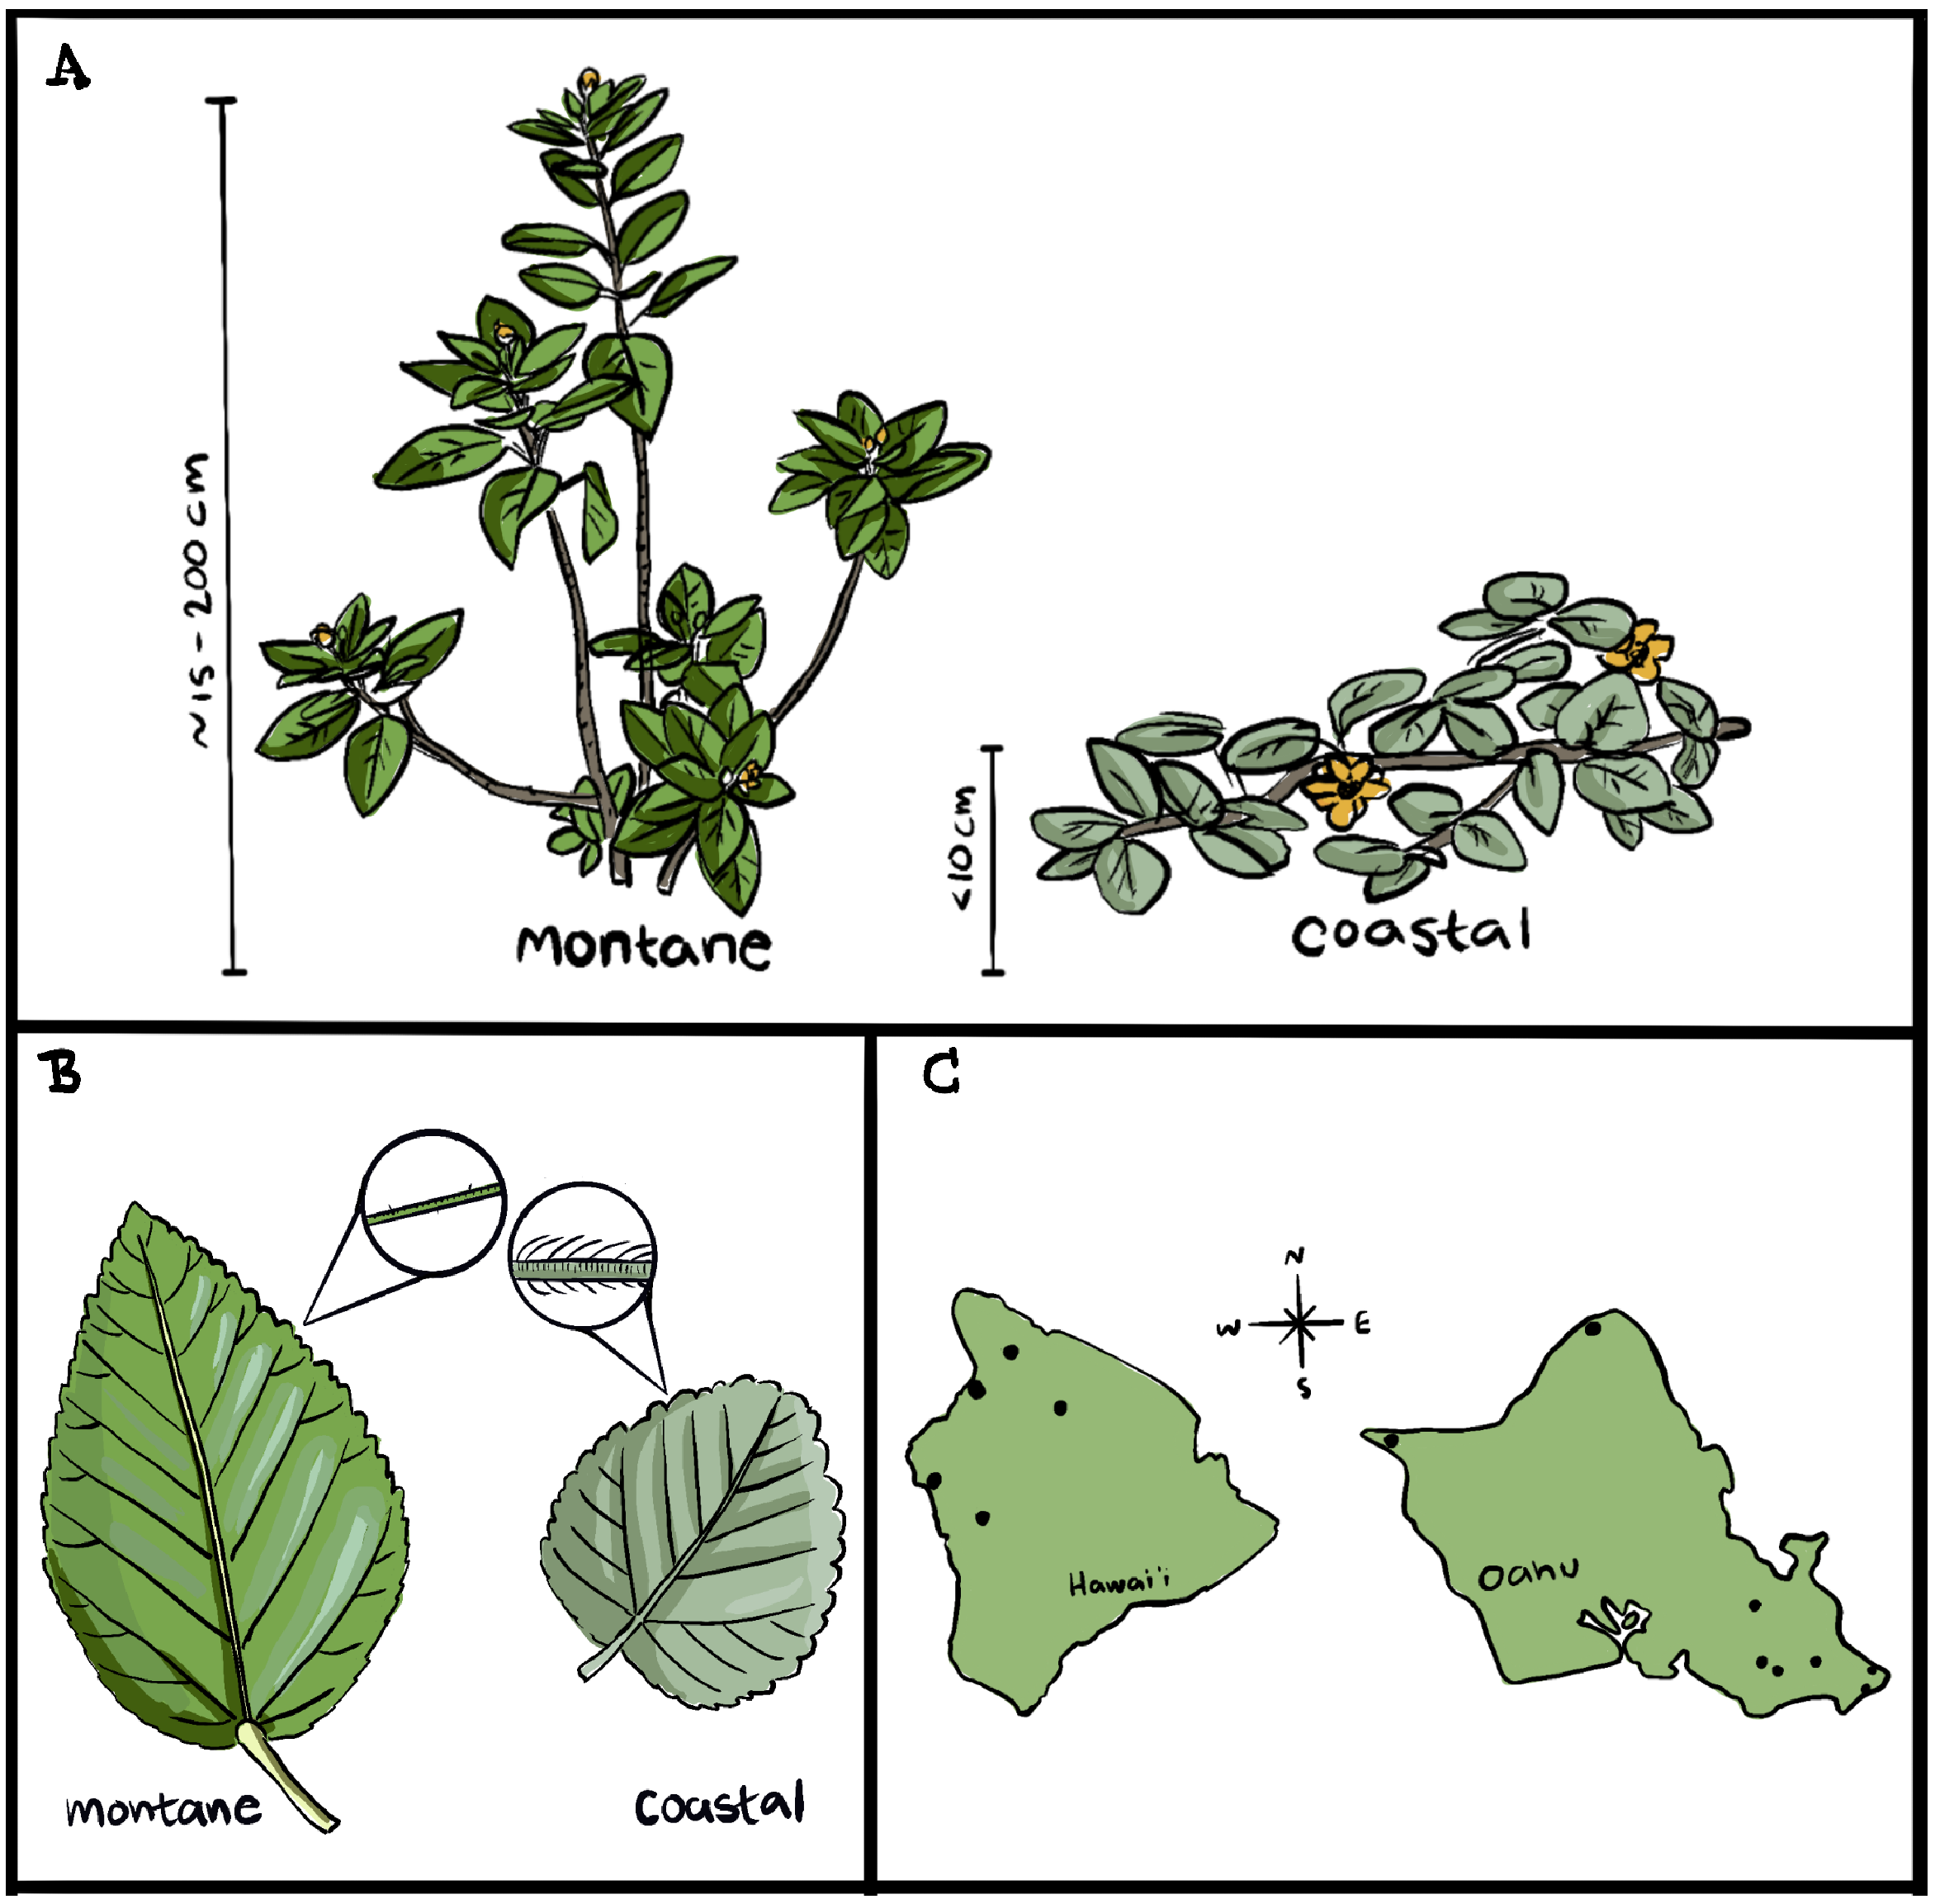
\includegraphics[height=3.25in]{../figures/study-system.pdf}
  % 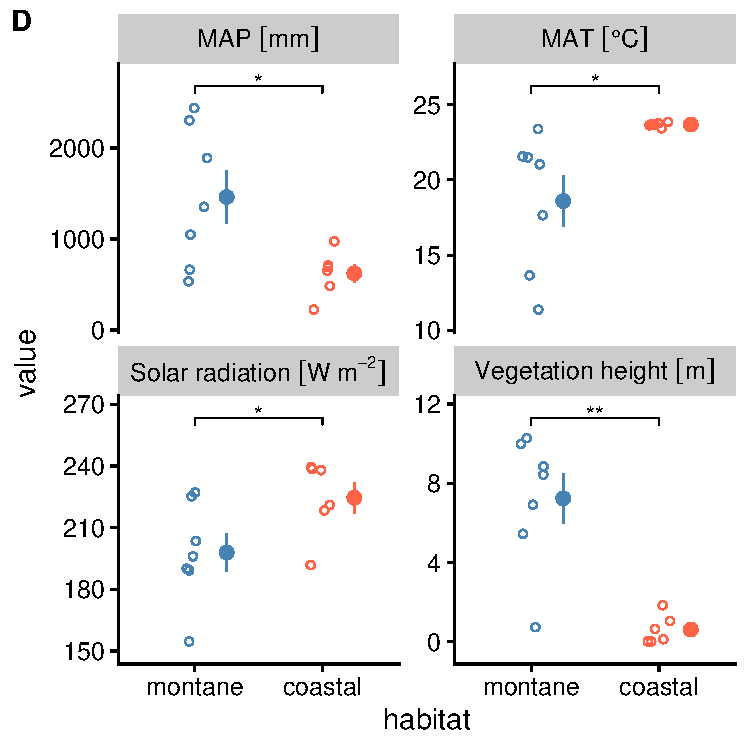
\includegraphics[height=3.25in]{../figures/habitat-climate.pdf}
  \caption{A. Typical growth form of montane (left) and coastal (right) ‘ilima plants and B. leaves. C. Map of the sites that were sampled on the islands of Oʻahu and Hawaiʻi (aka Big Island). D. Climatic, light, and vegetation height comparisons between montane (blue) and coastal (orange) habitats sampled in this study. Open circles are values for the midpoint of each site transect; closed circles and intervals are the mean $\pm~1$ standard error. The habitats differ significantly in mean annual precipitation (top-left), solar radiation (bottom-left), temperature (top-right), and vegetation height (bottom-right). MAP = mean annual precipitation; MAT = mean annual temperature; ns = not significant; * indicates $0.01 \le P < 0.05$; ** indicates $0.001 \le P < 0.01$.}
  \label{fig:study-system}
\end{figure}

\begin{figure}[H]
  % 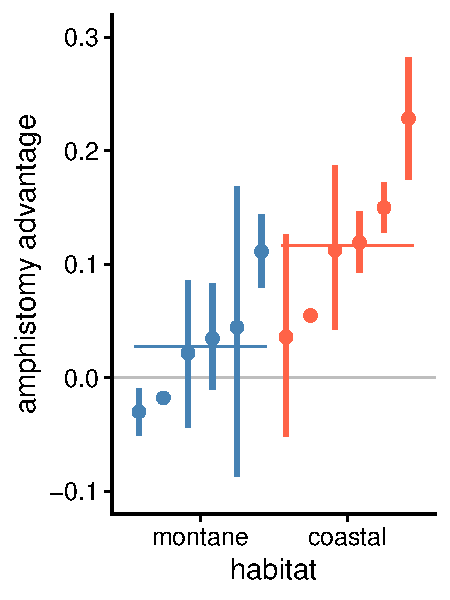
\includegraphics{../figures/habitat-aa.pdf}
  \caption{Coastal leaves benefit more from amphistomy than montane leaves. A positive amphistomy advantage ($y$-axis) means that the photosynthetic rate of an amphistomatous leaf is greater than that of an identical pseudohypostomatous leaf at the same overall $g_\mathrm{sw}$. Each point-interval is the median posterior estimate plus 95\% confidence interval of amphistomy advantage for that leaf. Each leaf is from a different montane (blue) or coastal (orange) site, arranged by habitat and ascending amphistomy advantage within habitat. The longer horizonal bars are the average amphistomy advantage for montane and coastal leaves. $g_\mathrm{sw}$, stomatal conductance to water vapor.}
  \label{fig:habitat-aa}
\end{figure}

\begin{figure}[H]
  % 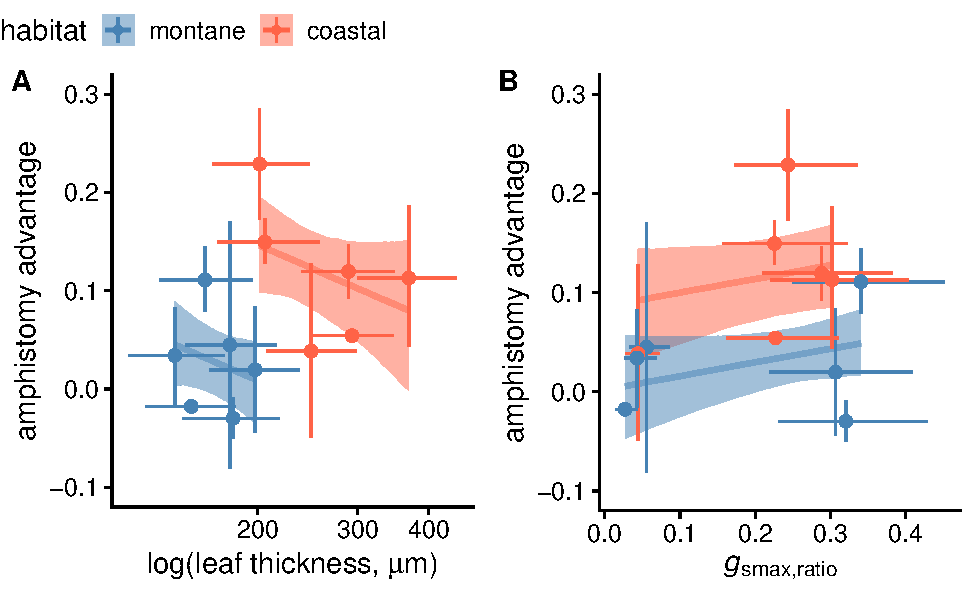
\includegraphics{../figures/traits-aa.pdf}
  \caption{Relationships between leaf amphistomy advantage, (A) leaf thickness and (B) $g_\mathrm{smax,ratio}$ among ʻilima (\textit{Sida fallax}) plants from montane (blue) and coastal (orange) habitats in Hawaiʻi. A positive amphistomy advantage ($y$-axis) means that the photosynthetic rate of an amphistomatous leaf is greater than that of an identical pseudohypostomatous leaf at the same overall $g_\mathrm{sw}$. Each point-interval is the median posterior estimate plus 95\% confidence interval of the trait value. Each leaf is from a different montane (blue) or coastal (orange) site. Lines are the estimated linear regression of (A) log(leaf thickness) and (B) $g_\mathrm{smax,ratio}$ on amphistomy advantage; ribbons are the 95\% confident bands of the regression. Symbols: $g_\mathrm{smax,ratio}$, anatomical maximum stomatal conductance ratio; $g_\mathrm{sw}$, stomatal conductance to water vapor.}
  \label{fig:traits-aa}
\end{figure}

\renewcommand\thefigure{S\arabic{figure}}    
\renewcommand\thetable{S\arabic{table}}    
\renewcommand\theequation{S\arabic{equation}}    
\setcounter{figure}{0}    
\setcounter{table}{0}    
\setcounter{equation}{0}

\begin{figure}
  \captionsetup{labelformat=empty}
  \caption{}
  \label{fig:ags-curve}
\end{figure}

\begin{figure}
  \captionsetup{labelformat=empty}
  \caption{}
  \label{fig:licor}
\end{figure}

\begin{figure}
  \captionsetup{labelformat=empty}
  \caption{}
  \label{fig:pp-licor}
\end{figure}

\begin{figure}
  \captionsetup{labelformat=empty}
  \caption{}
  \label{fig:habitat-Ags}
\end{figure}

\begin{figure}
  \captionsetup{labelformat=empty}
  \caption{}
  \label{fig:habitat-gmaxratio}
\end{figure}

\begin{table}
  \captionsetup{labelformat=empty}
  \caption{}
  
\end{table}



\end{document}
